\chapter{Foundations for inference} 
\label{foundationsForInference}

The United States Center for Disease Control and Prevention (CDC) focuses ``on policy and environmental strategies to make healthy eating and active living accessible and affordable for everyone.'' \footnote{\url{http://www.cdc.gov/obesity/}} One of the CDC's top priorities is understanding national obesity. A Body mass index (BMI) captures a person's height and weight within one measurement -- a high BMI indicates high body fat. The World Health Organization (WHO) classifies adults as underweight, healthy weight, overweight, and obese according to BMI. Below is a categorization provided by the WHO. \footnote{\url{http://apps.who.int/bmi/index.jsp?introPage=intro_3.html}}

\begin{center}
\begin{tabular}{|c|c|}
\hline 
Category & BMI range\tabularnewline
\hline 
\hline 
Underweight & $<18.50$\tabularnewline
\hline 
Normal (healthy weight) & 18.5-24.99\tabularnewline
\hline 
Overweight & $\geq 25$\tabularnewline
\hline 
Obese & $\geq30$\tabularnewline
\hline 
\end{tabular}
\end{center}

These policy makers are interested in the following questions: What is the average population BMI for adults in the United States? Instead of providing a single number, what is a reasonable range for the average U.S. adult BMI? Finally, is the average adult BMI in 2000 different than the average BMI 20 years ago?

These questions encompass the general ideas for statistical inference covered in Chapter \ref{foundationsForInference}. Inference is a set of tools used to estimate properties of a population, also known as parameters, after observing a sample from the population. Inference allows for different levels of confidence for these property estimates. Once they estimate the average adult BMI in the United States from a sample, scientists can ask how confident are they that this estimate is representative of the U.S. adult population. A classic inferential question is, ``How likely is it that the estimated mean, $\overline{x}$, is near the population mean, $\mu$?'' Statistical inference includes asking these questions but also determining which estimates to use.

Chapter \ref {foundationsForInference} provides the groundwork for inference on a population from observing one sample. Later chapters will cover inference comparing two or more distinct populations. The equations and details change depending on the setting, but the foundations and general procedures are the same throughout statistical inference. Understanding how to make inferences using one sample in this chapter will provide familiarity for more sophisticated methods in upcoming chapters. 

%__________________
\section{BRFSS data}
\label{brfssData}
The Behavioral Risk Factor Surveillance System (BRFSS), organized by the CDC and started in 1984, is the world's largest on-going telephone health survey system. This survey is nationwide and aims to ``monitor state-level prevalence of major behavioral risks among adults associated with premature morbidity and mortality.'' \footnote{\url{http://www.cdc.gov/brfss/about/about_brfss.htm}} Questionnaire topics include smoking, alcohol use, diet and exercise. The annual survey data from 2000, \data{BRFSS}, could be used to estimate the average adult BMI of the US population. The four variables\footnote{There are a total of 289 variables in the dataset.} that the CDC is interested in are listed in Table  ~\ref{brfssBMIVariables}. 


\begin{comment} http://www.cdc.gov/brfss/annual_data/annual_2000.htm#information\end{comment}
\begin{table}[h]
\centering\small
\begin{tabular}{l p{65mm}}
\hline
{\bf variable} & {\bf description} \\
\hline
\var{sex} & Male or Female where 1 is Male and 2 is Female\\
\var{age} & In years \\
\var{height} & In feet and inches where, for example, 5' 5" is listed as 505 \\
\var{weight} & In pounds\\
\end{tabular}
\caption{Variables of interest and their descriptions  from the \data{BRFSS} data set.}
\label{brfssBMIVariables}
\end{table}

BMI is not one of the variables listed, but BMI can be calculated from a person's height and weight. The calculation of BMI using both Metric and Imperial is \[BMI=\frac{\mathrm{weight_{kg}}}{\mathrm{height_{m}}^2}=\frac{\mathrm{weight_{lb}}}{\mathrm{height_{in}}^2}\cdot 703\]
where $\mathrm{weight_{kg}}$ and $\mathrm{height_{m}}$ are the weight and height measured in kilograms and meters respectively, and $\mathrm{weight_{lb}}$ and $\mathrm{height_{in}}$ are the weight and height in pounds and inches respectively. 

The CDC infers the average BMI of adults in the United States, the target population. A target population is the group that the statistician hopes to understand. Through inference, the statistician draws conclusions about the target population. 

The \data{BRFSS} dataset contains170,000 observations.  A simple random sample of 40 adults from the \data{BRFSS} data is taken and used by the CDC as the observed sample. \footnote{The CDC, after collecting the data, edited, processed, and weighted the raw data to make the values appear like they were drawn from a simple random sample of the U.S. adult population. Noncoverage and nonresponse become equal among all groupings of the population. The \data{BRFSS} data are this post-processed data. A simple random sample from \data{BRFSS} allows all observations an equal chance of being selected. The weighting formulae can be found at \url{http://www.cdc.gov/brfss/annual_data/2010/pdf/overview_10.pdf} under the Data Processing section.} This simple random sample of 40 adults from \data{BRFSS} (\data{BRFSS BMI}) will be used to draw conclusions about the target population, U.S. adults. Part of this dataset, including the BMI calculation, is shown in Table~\ref{brfssBMIData}. 

% latex table generated in R 3.1.1 by xtable 1.7-4 package
% Fri Oct  9 05:04:04 2015
\begin{table}[ht]
\centering
\begin{tabular}{rrrrrr}
  \hline
 & sex & age & height & weight & BMI \\ 
  \hline
1 &   2 &  60 & 508 & 200 & 30.41 \\ 
  2 &   2 &  25 & 506 & 145 & 23.40 \\ 
  3 &   1 &  40 & 511 & 180 & 25.10 \\ 
  4 &   1 &  53 & 511 & 210 & 29.29 \\ 
  5 &   2 &  80 & 504 & 170 & 29.18 \\ 
  6 &   2 &  71 & 501 & 108 & 20.40 \\ 
   \hline
\end{tabular}
\caption{Six observations from the \data{BRFSS BMI} dataset} 
\label{brfssBMIData}
\end{table}

Strictly speaking, \data{BRFSS} is the target population when using the \data{BRFSS BMI} sample because the 40 observations were not a simple random sample from the U.S. adult population but a simple random sample from \data{BRFSS} instead. However if the \data{BRFSS} dataset is a reasonable surrogate for the U.S. population, \footnote{We believe so.} then drawing samples from \data{BRFSS}'s 170,000 observations is equivalent to directly drawing from the U.S. adult population. This assumption is made in throughout the chapter going forward. In practice, the CDC would simply use all 170,000 observations as a single sample to make inference on the U.S. adult population.

Observing a random sample and drawing conclusions about the target population is the practice of statistical inference in the broadest sense, but the data should be explored graphically using the tools from Chapter~\ref{introductionToData} first. The histogram and box plot in Figure~\ref{exploreBMI} show that the sample is skewed right. The mean BMI of the sample is higher than the median of the sample. Foundations and methods of statistical inference follow naturally after the data have been examined and explored. 

\begin{figure}
\centering
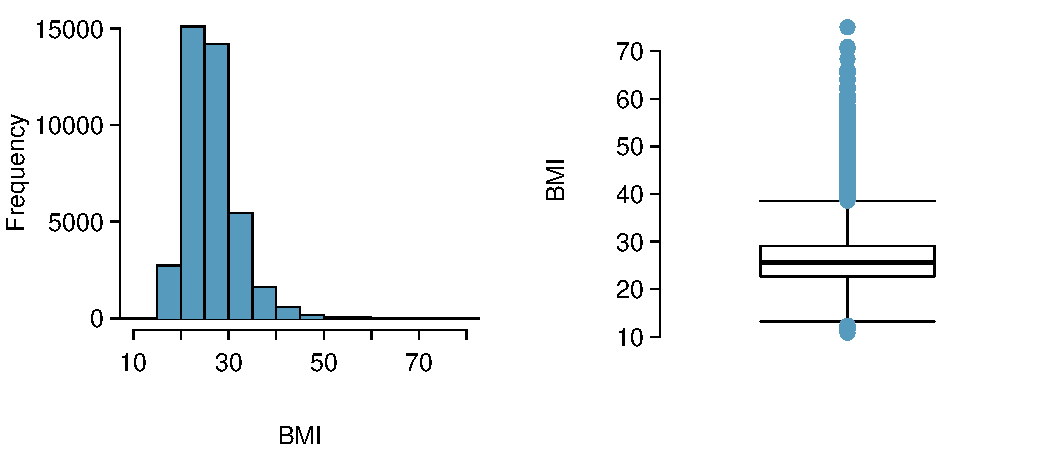
\includegraphics[width =  \textwidth]{ch_inference_foundations_oi_biostat/figures/brfssBMIsampHistograms/brfssBMIsampHistograms}
\caption{Histogram and boxplot of \var{BMI} for the \data{BRFSS BMI} data. The data is skewed right.}
\label{exploreBMI}
\end{figure}

%__________________
\section{Mechanics of inference}
\label{mechanicsofInference}

Chapter~\ref{foundationsForInference} introduces two forms of estimation for the population average: a point estimate and a confidence interval. A point estimate is a single number that best estimates the average adult BMI in the United States. A confidence interval is a range of values that best captures the average U.S. adult BMI at some confidence level. The confidence interval does not guarantee the inclusion of the population parameter. 

\data{BRFSS BMI}, a sample of 40 observations, has a sample mean of 26.53, and a sample standard deviation of 5.84. The point estimate for the population average is 26.53, the sample mean, $\overline{\mathrm{BMI}}$. With 95\% confidence, the CDC calculates the confidence interval as
\begin{eqnarray}
\text{point estimate}\ \pm\ 2 \times SE \\
\overline{\mathrm{BMI}}\ \pm\ 2 \times \frac{s}{\sqrt{n}}\\
26.53\ \pm\ 2 \times \frac{5.84}{\sqrt{40}}\\
(24.68, 28.38)
\label{95PercentConfidenceIntervalFormula}
\end{eqnarray}

where $s$ is the sample standard deviation, $n$ is the number of observations within the sample and $\overline{\mathrm{BMI}}$ is the point estimate. 

The calculation of these estimates is straightforward and mechanical. The steps involved in hypothesis testing are equivalently formulaic. Understanding what these estimates represent, why they are calculated as they are, and how they relate to one another is even more foundational. 

Section~\ref{variabilityInEstimates} introduces the point estimate and its particular flaw: ignoring point estimate variability. Sampling variability is difficult to observe from a single observation, but Section~\ref{pointEstimates} and Section~\ref{sampDist} illustrate through \textsf{R} and repeated sampling that such variation exists. 

Section~\ref{confidenceIntervals} presents the confidence interval to incorporate variability and dissects the formula \[\text{point estimate}\ \pm\ 2 \times SE\] to fully understand each of its terms. These opening sections will explore the theory and motivate point estimates and confidence intervals empirically through \textsf{R}. These estimation techniques are fundamental in mastering hypothesis testing, presented in Section~\ref{hypothesisTesting}.

%__________________
\section{Variability in estimates}
\label{variabilityInEstimates}

\index{point estimate|(}

If the CDC, after observing the \data{BRFSS BMI} sample, were asked to give its best guess for the average adult BMI in the U.S., what would it be? The CDC would provide a point estimate. A \term{point estimate} is a single value derived from sample data that serves as the ``best guess'' for that population parameter. Section~\ref{variabilityInEstimates} looks at point estimates and the variability inherent in using a single number as the best guess.\footnote{This chapter begins with inference on the population mean but questions regarding variation are often just as important. For instance, potential action regarding obesity could change if the standard deviation of the average adult BMI were 5 versus if it were 15.} 

\subsection{Point estimates}
\label{pointEstimates}

A likely choice to estimate the \term{population mean} is to take the \term{sample mean}. That is, use the average BMI in the \data{BRFSS BMI} sample as the estimate for the BMI among U.S. adults. 

For notation, use $\mathrm{BMI}_1, \mathrm{BMI}_2, \ldots, \mathrm{BMI}_{40}$  to represent the BMI for each survey respondent in the \data{BRFSS BMI} sample. The sample mean of \data{BRFSS BMI} is 
\begin{eqnarray*}
\overline{\mathrm{BMI}} = \frac{30.41 + 23.40 + 25.10 + \dots}{40} = 26.53
\end{eqnarray*}
\index{point estimate!single mean|(}
$\overline{\mathrm{BMI}}=26.53$ serves as the \term{point estimate} of the population mean. \footnote{If \var{weight} is the variable of interest instead, the sample mean of observations denoted $w_1,\ldots w_{40}$ would be $\overline{w}$}

What about generating point estimates of other \term{population parameters}, such as the population median or population standard deviation? Sample statistics can estimate these parameters as well. The population standard deviation for adult BMIs can be estimated using the sample standard deviation. The population median is estimated by the sample median. Table~\ref{BMIEstimates} provides the point estimates to other BMI population parameters using the \data{BRFSS BMI} sample.

% latex table generated in R 3.1.1 by xtable 1.7-4 package
% Fri Oct  9 05:32:46 2015
\begin{table}[ht]
\centering
\begin{tabular}{lr}
  \hline
BMI & estimates \\ 
  \hline
mean & 26.53 \\ 
  median & 25.93 \\ 
  std. dev. & 5.84 \\ 
   \hline
\end{tabular}
\caption{Point estimates for the \var{BMI} variable} 
\label{BMIEstimates}
\end{table}

\begin{exercise} \label{pointEstimateOfDesiredWeights}
The CDC wants to estimate the difference in the average age for U.S. adult men and women. If $\overline{\mathrm{age}}_{\mathrm{women}} = 50.22 $ years and $\overline{\mathrm{age}} _ {\mathrm{men}} = 47 $ years, what would be a reasonable point estimate for the age difference in the population? \footnote{Take the difference of the two sample means: $\overline{\mathrm{age}}_{\mathrm{women}} - \overline{\mathrm{age}} _ {\mathrm{men}} = 50.22 - 47 =  3.22$. Women are, on average, estimated to be older than men by 3.22 years.}
\end{exercise}
%men = brfss.sample[which(brfss.sample$sex == 1),]
%women = brfss.sample[which(brfss.sample$sex == 2),]
%mean(women$age) - mean(men$age)

\begin{exercise}
Provide a point estimate for the population IQR given the \data{BRFSS BMI} sample. \footnote{Use the IQR of a random sample from the population as the point estimate for the population IQR.}
\index{point estimate!single mean|)}

\end{exercise}

Suppose a different sample of 40 people is taken from \data{BRFSS} and the mean calculated; the answer will likely not be the same as $26.53$, the \data{BRFSS BMI} sample mean. There exists \term{sampling variation} within a point estimate. Estimates generally vary from one sample to another even among samples of the same size. The sample mean is the best guess for the population average, but it is most likely not equal to the population parameter. Low sampling variation can suggest that the estimate observed may be close to the population parameter, but as the population parameter is rarely ever known, there is no guarantee that the estimate is close. A larger sample size can, with high probability, produce a closer estimate to the population parameter than one taken from a smaller sized sample. 

\textsf{R} can be used to demonstrate sampling variation. Another simple random sample from the \data{BRFSS} data of 40 is taken. The new sample mean for the BMI could be 28.17. Doing this again, the average BMI could be 24.89. Estimates differ across samples through sampling variation, but in practice, it is extremely rare to observe more than one sample from a population.

A \term{running mean} -- a sequence of means where each mean uses one more observation in its calculation than the mean directly before it in the sequence -- demonstrates sampling variation and increasing precision for larger sample sizes. With \data{BRFSS BMI}, the second mean is the average of the first two observations, $\mathrm{BMI}_1, \mathrm{BMI}_2$. The third number in the sequence is the average of $\mathrm{BMI}_1, \mathrm{BMI}_2,$ and $\mathrm{BMI}_3$. 

The running mean from the \data{BRFSS BMI} sample is shown in Figure~\ref{BMIRunningMean}. As more observations are included, the running mean converges closer to 26.53, the sample mean. Similarly if the sample size increases from 40 to 100 observations, the sample mean from the larger sample should be closer to the average U.S. adult BMI than the sample mean with 40 observations. 

\begin{figure}
   \centering
   \includegraphics[width=\textwidth]{ch_inference_foundations_oi_biostat/figures/brfssBMIRunningMean/brfssBMIRunningMean}
   \caption{The running mean calculated from the \var{BRFSS BMI} sample of 40 observations. The mean stabilizes and approaches $\overline{\mathrm{BMI}} = 26.53$ as the number of observations increases to 40.}
      \label{BMIRunningMean}
\end{figure}

Sampling variation is across samples of the same size. Figure~\ref{runningSamplingVariation} displays the running means of two samples randomly drawn from \data{BRFSS} of size 40. There exists a substantial amount of sampling variation; the path of the running means are not the same at a small sample size.

Sampling variation decreases as the number of observations increases. Figure~\ref{runningSamplingVariation20} illustrates this more clearly by calculating the running means of 20 independent samples of 40 observations. The sampling variation is large with small sample sizes $n$, but as the number of observations increases toward 40, the variation among the running means decreases. 

\begin{figure}
   \centering
   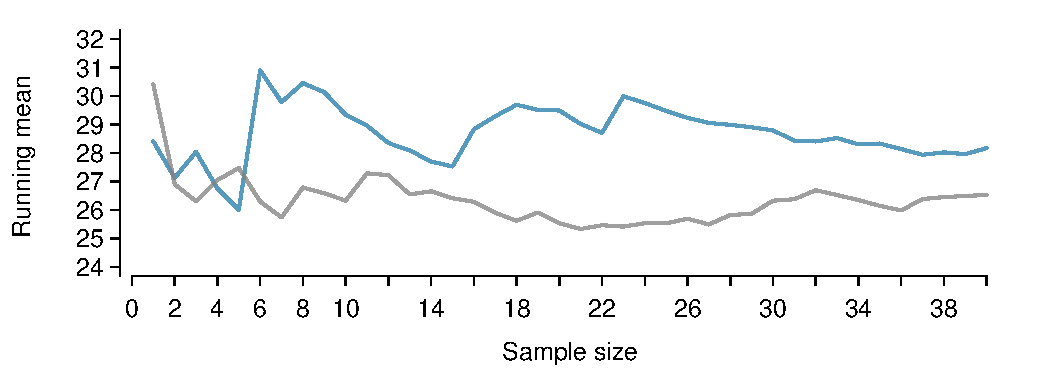
\includegraphics[width=\textwidth]{ch_inference_foundations_oi_biostat/figures/brfssBMISampVar/brfssBMISampVar}
   \caption{The running means of two samples drawn from \data{BRFSS}. The gray line is the running mean from \data{BRFSS BMI}. The blue line is the running mean from a different sample drawn randomly from \data{BRFSS}. The exists high sampling variation at the beginning but as the sample size increases, the running means converge.}
	\label{runningSamplingVariation}
\end{figure}

\begin{figure}
   \centering
   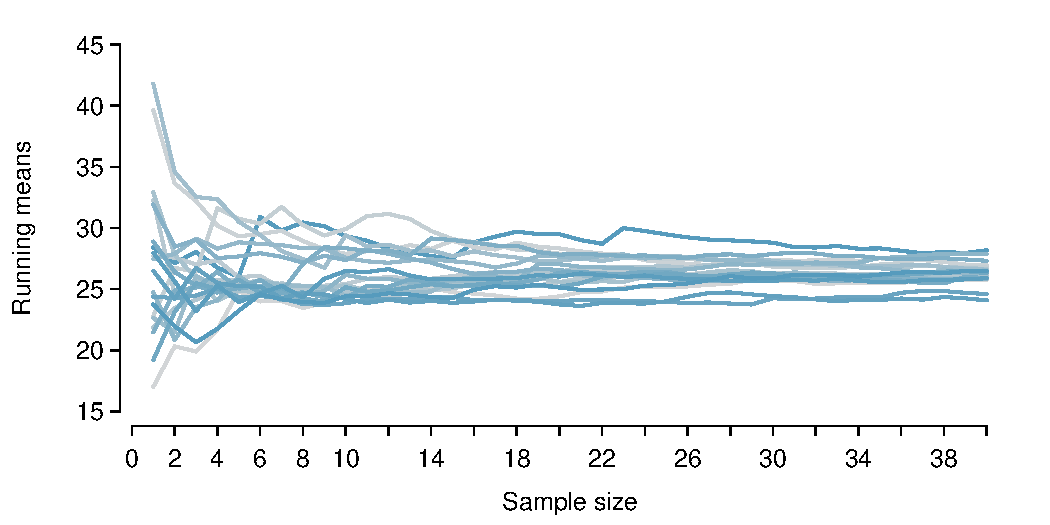
\includegraphics[width=\textwidth]{ch_inference_foundations_oi_biostat/figures/brfssBMISampVar/brfssBMISampVar20}
   \caption{The sampling variation among the 20 running means decreases as the number of observations gets larger.}
	\label{runningSamplingVariation20}
\end{figure}

Sampling variation at different sample sizes also serves as evidence. Figure ~\ref{sampleMeanPrecision} shows two histograms of sample means for samples taken from \data{BRFSS}. The sample means in the left histogram and right histogram have sample sizes of five and 40 respectively. The histogram with $n=40$ has noticeably smaller variance than the histogram with $n=5$. Section ~\ref{seOfTheMean} demonstrates how to quantify and measure sampling variation as more data becomes available. 

\begin{figure}
   \centering
   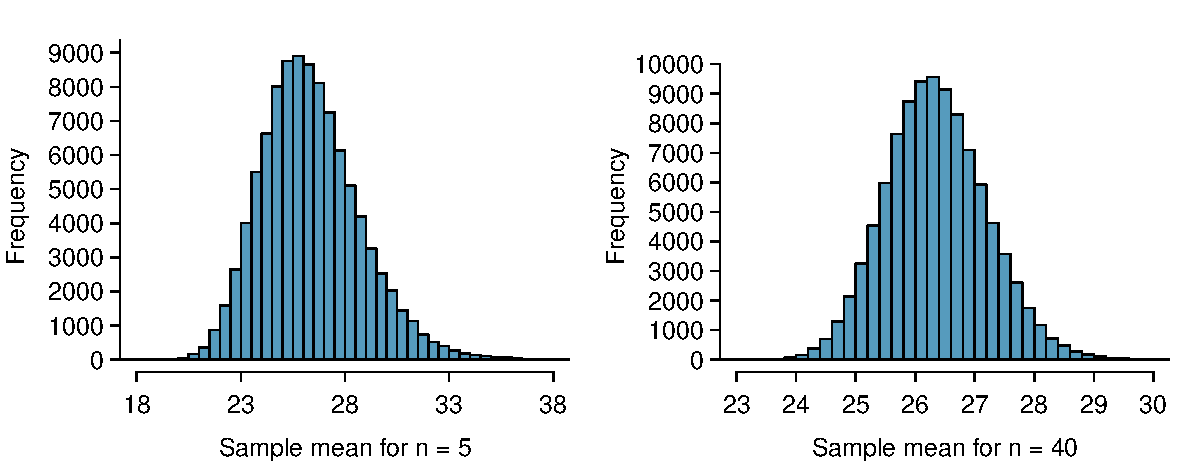
\includegraphics[width=\textwidth]{ch_inference_foundations_oi_biostat/figures/brfssBMISampleMeanPrecision/brfssBMISampleMeanPrecision}
   \caption{Sample means of size $n=5$ and $n=40$. The histogram with $n=40$ has a smaller variance.}
   \label{sampleMeanPrecision}
\end{figure}

Beyond spread, the histogram with $n=5$ is also slightly skewed, but both appear to be centered approximately around the same value. Another characteristic of the sample mean is that it does not contain any systematic error or bias. The center of the running means in Figure ~\ref{runningSamplingVariation20} and the histograms in Figure ~\ref{sampleMeanPrecision} are, on average, the population average BMI. Section ~\ref{aFrameworkForInference} discusses other unbiased point estimates beyond the sample mean used for statistical inference.
 
\subsection{Sampling variability and sampling distribution}
\label{sampDist}

\data{BRFSS BMI} is one random sample from \data{BRFSS} with one sample mean, $26.53$. Another random sample of 40 was taken from \data{BRFSS} in Section ~\ref{pointEstimates} and its mean calculated, $28.17$. This happens again (24.89) and again (26.34), and continue to do this many many times. \footnote{These values were calculated from resampling the \data{BRFSS} data in \textsf{R}. These particular numbers are some of many possible values a sample mean can take on, depending on the sample itself.} Repeated sampling is only possible with access to  the\data{BRFSS} data. This procedure generates an approximation to the \term{sampling distribution} for the sample mean of sample size 40, shown in Figure~\ref{brfssBMISamplingDistribution}.\footnote{The sampling distribution is constructed by repeated sampling from the target population. While \data{BRFSS} is not quite the target population of U.S. adults, the 170,000 observations are a large enough sample to be a representative substitute for the target population.} 

\begin{termBox}{\tBoxTitle{Sampling distribution}
The \term{sampling distribution} is the distribution of a point estimate based on samples of a fixed size from a certain population. A point estimator has an associated unique sampling distribution. Understanding the concept of a sampling distribution is central to understanding variability and statistical inference.}
\end{termBox}

\begin{figure}
   \centering
   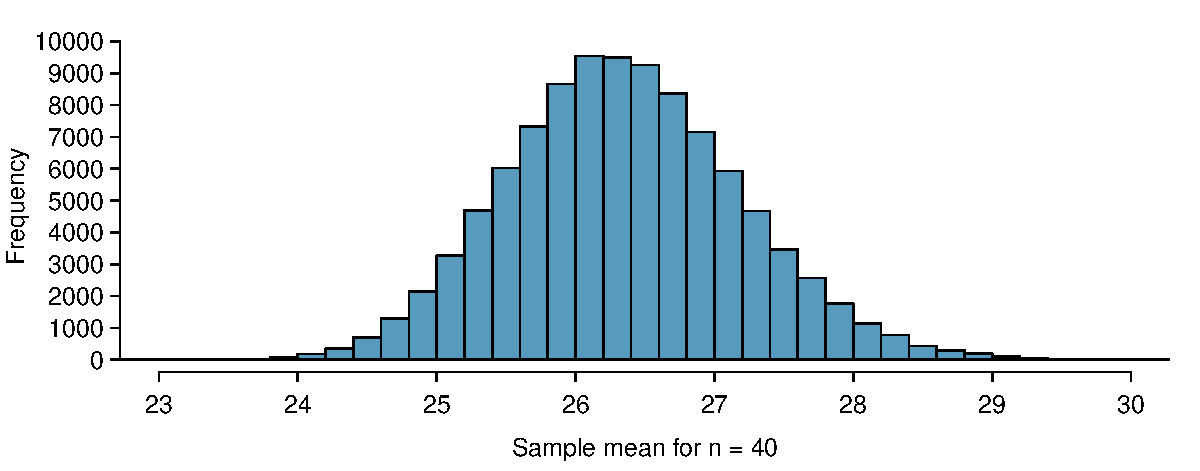
\includegraphics[width=\textwidth]{ch_inference_foundations_oi_biostat/figures/brfssBMISamplingDistribution/brfssBMISamplingDistribution}
   \caption{A histogram of an approximation to the sampling distribution. Here 100,000 sample means for BMI were calculated, where the samples are of size $n=40$. }
      \label{brfssBMISamplingDistribution}
\end{figure}

Figure~\ref{brfssBMISamplingDistribution} is an approximation of the sampling distribution. A point estimate from a particular sample of said size is one observation in the sampling distribution. In almost all cases, the sample distribution is unobservable beyond the single point estimate from the sample the scientists observe. \footnote{To get an exact sampling distribution, the sample means from every possible unique combination of 40 respondents in the U.S. adult population (and not from the \data{BRFSS} dataset) needs to be calculated. The CDC would never create a sampling distribution and instead would use all 170,000 observations to calculate one sample mean.}The sampling distribution, however, is a fundamental concept that illustrates sampling variability. 
 
An approximation of the sampling distribution of the sampling mean can be created using \data{BRFSS} and sampling variation illustrated with the following pseudocode: 

\begin{verbatim}
(1) Create a vector to store the sample mean values once calculated
(2) Take a sample of 40 from BRFSS
(3) Calculate the sample mean of BMI values and store the sample mean in (1)
(4) Repeat (2) and (3) many many times 
(5) Plot the vector of sample means as a histogram 
\end{verbatim}
  
The sampling distribution for the sample mean is unimodal and symmetric, centered at the target population's mean. The sample mean is, intuitively, the best guess for the population mean. The sample means should tend to ``fall around'' the mean of the target population.

\subsection{Standard error of the mean}
\label{seOfTheMean}

Variability exists among point estimates. The average adult BMI ranged from 24 to 29 in Figure ~\ref{brfssBMISamplingDistribution} for samples of size 40. Variability decreases for larger sample sizes. Section ~\ref{pointEstimates} suggests that there should exist some metric, dependent on sample size, to quantify the variability of a point estimate.

\begin{tipBox}{\tipBoxTitle{More data means less variability}
In sampling, the larger the sample size the better. The precision of the sample mean increases as more data is observed within a sample.}
\end{tipBox}

Standard deviation is an obvious method to quantify variability. The standard deviation of the sample mean indicates how far the typical estimate is away from the population mean. IStandard deviation is a very good metric to size the typical \term{error} of the point estimate, and for this reason, an estimate's standard deviation is called the \term{standard error (SE)} \index{SE}\marginpar[\raggedright\vspace{-4mm} $SE$\\\footnotesize standard\\error]{\raggedright\vspace{-4mm} $SE$\\\footnotesize standard\\error} of the estimate. 

\begin{termBox}{\tBoxTitle{Standard error of an estimate}
The standard deviation associated with an estimate is called the \emph{standard error}. It describes the typical error or uncertainty associated with the estimate.}
\end{termBox}

The standard error of the estimate is a measure of spread among the possible estimates, which are drawn from the sampling distribution. The standard deviation of the sampling distribution, denoted  $\sigma_{\overline{x}}$, serves as a reasonable measure of a point estimate's variability.

\begin{tipBox}{\tipBoxTitle{"Standard Deviation" $\neq$ "Standard Error"}
Caution: The standard deviation of the sample mean is not equivalent to the estimate for the population standard deviation. The term "standard error" is not interchangeable with "standard deviation." Standard deviation describes the spread of values within one sample. The standard error of the sample mean describes how accurate the sample mean is to the population mean. It represents the spread among all sample means. These two terms are measuring two separate quantities.}
\end{tipBox}

\begin{exercise}
(a) Which one achieves a "better" estimate of a parameter: using a small sample or a large sample? Why? (b) Using the same reasoning from (a), is a point estimate based on a small sample expected to have smaller or larger standard error than a point estimate based on a larger sample?

\footnote{(a) Prefer a large sample. Consider two random samples: one of size 10 and one of size 1000. Individual observations in the small sample are highly influential on the estimate while in larger samples these individual observations would more often "average each other out." The larger sample would tend to provide a more precise estimate of the parameter. (b) A "better" estimate typically means it has less error. Based on (a), intuition suggests that a larger sample size corresponds to a smaller standard error. In general the standard error, or variability, for an estimate gets smaller as the samples get larger.}
\end{exercise}

The standard deviation of the sampling distribution is difficult to compute since the sampling distribution is unobservable. Through repeated sampling, an approximation of the sampling distribution serves as a substitute. The standard deviation of the calculated sample means from Section~\ref{sampDist} pseudocode serves as the estimate for the standard error. The algorithm in \textsf{R} is below:\footnote{This computing experience samples without replacement to simulate sampling in the real world (researchers would never sample the same person twice), however standard errors would never be calculated through simulation. Theory, instead, requires individual BMI values to be independent. A reliable method to ensure independence is to use the 10\% rule of thumb: observations from simple random samples with a size less than 10\% of the population are considered independent. Sampling without replacement within a finite population still results in a reasonable estimate for the standard error.}

\begin{verbatim}
N <-10000 #the number of iterations to do
sample.means<- array(data=NA,dim = N) #to store the sample means
for(i in 1:N){
  #take a sample of size 40 from the BRFSS dataset without replacement
  #BRFSS is the dataset and $BMI only calls the "BMI" column from the BRFSS dataset
  sample<-sample(x=BRFSS$BMI, size=40, replace=FALSE) 
  
  #calculate the mean of the sample and store it 
  sample.means[i]<-mean(sample)
}

#standard deviation of the approximation to the sampling distribution
#serves as the estimate of the standard error
sd(sample.means) 
\end{verbatim}

The estimated standard error, \data{sd(sample.means)}, of a simulation with 10,000 sample means is $0.83$. This method, however, has one underlying problem: most often, scientists observe only one sample mean, $\overline{x}$. They cannot repeatedly sample. What do they do? The standard error of the sample mean can be calculated from a single sample with the following equation:

\begin{termBox}{\tBoxTitle{Calculating SE for the sample mean}
Given $n$ independent observations from a population with standard deviation $\sigma$, the standard error of the sample mean is equal to \vspace{-1mm}
\begin{eqnarray}
SE_{\text{ sample mean}} = \frac{\sigma}{\sqrt{n}}
\label{seOfXBar}
\end{eqnarray}\vspace{-3mm}%

A reliable method to ensure sample observations are independent is to guarantee that the sample from the population is a simple random sample with a size that is less than 10\% of the population size.\index{standard error!single mean}
}
\end{termBox}

There is one subtle issue of Equation~(\ref{seOfXBar}): the population standard deviation is typically unknown. Section \ref{pointEstimates} suggests that the``best guess'' for the population standard deviation, the sample standard deviation, can be used as a substitute. This estimate tends to be sufficiently good when the sample size is at least 30 and the population distribution is not strongly skewed. Practitioners then replace $s$ for $\sigma$ in Equation ~\ref{seOfXBar}. When the sample size is smaller than 30 or the skew condition is not met, a larger sample or other methods need to be used. These topics are further discussed in Section~\ref{cltSection}. 

The standard error of the sample mean from observing \data{BRFSS BMI} is 

\begin{eqnarray*}
SE_{\overline{x}} = \frac{s}{\sqrt{n}} = \frac{5.84}{\sqrt{40}} =  0.92
\end{eqnarray*}
where $s$ is the standard deviation of the sample and $n$ is the number of observations in the sample. The calculated standard error  $(0.92)$ is similar to the empirical standard deviation that was calculated from the sampling distribution $(0.83)$ \footnote{For context, the sample taken in Section ~\ref{pointEstimates} with sample mean 28.17 results in a standard error of $8.85/\sqrt{40} =1.40$. Variability also exists within sample standard deviations.}. 

\begin{exercise}
In another sample of 40 U.S. adults, the standard deviation of the sample is $s_\mathrm{BMI} = 4.81$. The sample is a simple random sample of less than 10\% of the United States population. The observations are independent. (a)~What is the standard error of the sample mean, $\overline{BMI}$? (b)~Is it surprising if the CDC published a report with the average BMI of all US adults as 30 after observing a sample mean of 26.36? How about 25?

\footnote{(a) Use Equation~(\ref{seOfXBar}) with the sample standard deviation to compute the standard error: $SE_{\overline{\mathrm{BMI}}} = 4.81/\sqrt{40} =  0.76$. (b) It is surprising if the average adult BMI of the US population was 30. A BMI of 30 is many many standard deviations away ($SE=0.76$) from the sample mean of 26.36. 
A BMI of 25 is less than one standard deviation away from the estimated population mean. The report would be less surprising. }
\end{exercise}

\begin{exercise}
(a) Are the results of a sample of 100 or 400 observations more trusting? (b) If the standard deviation of the individual observations is 10, what is the estimate of the standard error when the sample size is 100? What about when it is 400? (c) Explain how your answer to (b) mathematically justifies your intuition in part~(a).

\footnote{(a) Look back to Section ~\ref{pointEstimates} on sampling variation and more data. Extra observations are helpful in understanding the population, so a point estimate with 400 observations seems more trustworthy. (b) The standard error when the sample size is 100 is given by $SE_{\bar{x}_100} = 10/\sqrt{100} = 1$. For 400: $SE_{\bar{x}_400} = 10/\sqrt{400} = 0.5$. The larger sample has a smaller standard error if the sample standard deviations were the same. Estimates tend to be more precise when the sample size is larger. (c) The standard error, the typical error between the estimate and the population parameter, of a sample with 400 observations is lower than for a sample with 100 observations with equal sample standard deviations. The math in (b) shows that estimates from a larger sample tend to have smaller standard errors, though it does not guarantee that every large sample will provide a better estimate than a particular small sample.} 
\end{exercise}

\subsection{Basic properties of point estimates}

This section achieved three goals. First, point estimates from a sample are single numbers used to estimate population parameters. Furthermore, there exists sampling variation for point estimates. Because researchers only have the capacity to observe a single sample, it is not obvious that point estimates contain variability. The sampling distribution, a theoretical and fundamental concept, justifies the existence of sampling variation through its many possible sample estimates. Lastly, standard error quantifies sampling variation, which can be mathematically calculated from Equation~\eqref{seOfXBar}. Point estimates and their standard errors can be quantified for other parameters  -- the median, standard deviation, or any other number of statistics. These extensions will be postponed until later chapters and courses.

\index{point estimate)}

%__________________
\section{Confidence intervals}
\label{confidenceIntervals}

\index{confidence interval|(}

\subsection{Capturing the population parameter}

Using only a point estimate is like fishing in a murky lake with a spear. Fishermen who fish with spears will probably miss. Using a confidence interval is like fishing in the same lake with a net. If fishermen use nets in that area, they are more likely to catch a fish. 

Similarly, a point estimate provides a single value as the "best guess" for a parameter. It is rarely perfect and exact; usually there is error in the estimate. The standard error conveys how large this sampling variation is but a single point estimate alone does not. It lacks information about the standard error. Is there a measurement that conveys a point estimate's value and its sampling variation simultaneously? 

If a range of plausible values is reported -- \term{a confidence interval} -- it becomes more likely that the parameter is captured or contained within such range. The range incorporates sampling variation through the width of the interval. The larger the interval generally indicates the large the sampling variation and standard error \footnote{It could also indicate the higher confidence level. This will be introduced later}. As with fishing, the goal of the confidence interval is for the population parameter to be within the range.

\begin{exercise}
If we want to be very certain we capture the population parameter, should we use a wider interval or a smaller interval?\footnote{If we want to be more certain when capturing a fish, we might use a wider net. Likewise, we use a wider confidence interval if we want to be more certain that we capture the parameter. The more values included in the range, the more likely it is that this range contains the true value. The interval contains simply \emph{more} values. However capturing the parameter is not always the only goal when constructing a confidence interval. The parameter will always be captured with the widest interval going from $-\infty$ to $+\infty$ but this range does not increase understanding of the population parameter. } 
\end{exercise}
\begin{exercise}
Suppose a confidence interval is 10 units wide and we are 50\% confident that the range encompasses the population parameter. If another interval was instead 5 units wide centered at the same value as the original interval, are we now more or less confident than 50\% that the range will include the population parameter? \footnote{We are less than 50\% confident that the smaller interval includes the population parameter. Using a smaller net with fewer values, we are less confident that the population parameter is captured.}
\end{exercise}

\subsection{Confidence levels}
\label{confidenceLevels}

The size of a fishing net depends on how confident fishermen want to be in catching a fish. Similarly, a confidence interval width also changes with how confident scientists want to be in estimating the population parameter, but how is "confidence" defined?

Scientists first must choose a confidence level before the interval is constructed. Confidence levels, used even beyond confidence intervals, are associated with a level of uncertainty and how much the estimate procedure is allowed to commit a Type I Error or a false positive. Section~\ref{DecisionErrors} goes into more depth on Type 1 and Type 2 Errors. 

If the CDC says that it is 75\% confident that the adult population BMI is between two values, 75\% would be the measure of certainty and 25\% would be the probability of committing a Type 1 Error. In other words, there is a 25\% chance that the population parameter is not within the confidence interval. The Type I error is also known as $\alpha$.  

\begin{example}{Consider extreme confidence levels. What are the implications of a 100\% confidence level confidence interval? How about a 0.001\% confidence level?} \label{extremeConfidenceLevels}
A 100\% confidence level is equivalent to $\alpha = 0\%$. There is 0 chance that a Type 1 Error will be committed.The confidence interval created will \emph{always} capture the population parameter. To guarantee this, the confidence interval will be $[-\infty, \infty]$ . Consider a confidence level of 0.001\%. This extremely low confidence level results in a very high Type 1 Error. In many cases when building a 0.001\% confidence interval, the confidence interval will not capture the population parameter. Therefore this interval is expected to be extremely narrow. 
\end{example}

A 95\% confidence level is used most often in tradition \footnote{Section ~\ref{significanceLevel} demonstrates that any confidence level can be used} but what does "95\% confident" actually mean?

Suppose many samples were drawn and confidence intervals were built around each sample. To be 95\% confident, approximately 95\% of those intervals would contain the population parameter, $\mu$. If the CDC took 100 independent samples and built 100 confidence intervals at the 95\% confidence level for adult US BMI, 95 of these intervals would contain the average adult US BMI. Five of these would not.

Figure~\ref{95PercentConfidenceInterval} shows this process with 25 samples randomly drawn of 100 observations each, where 24 of the resulting confidence intervals contain the average BMI of \data{BRFSS} and one does not.

\begin{figure}[hht]
   \centering
   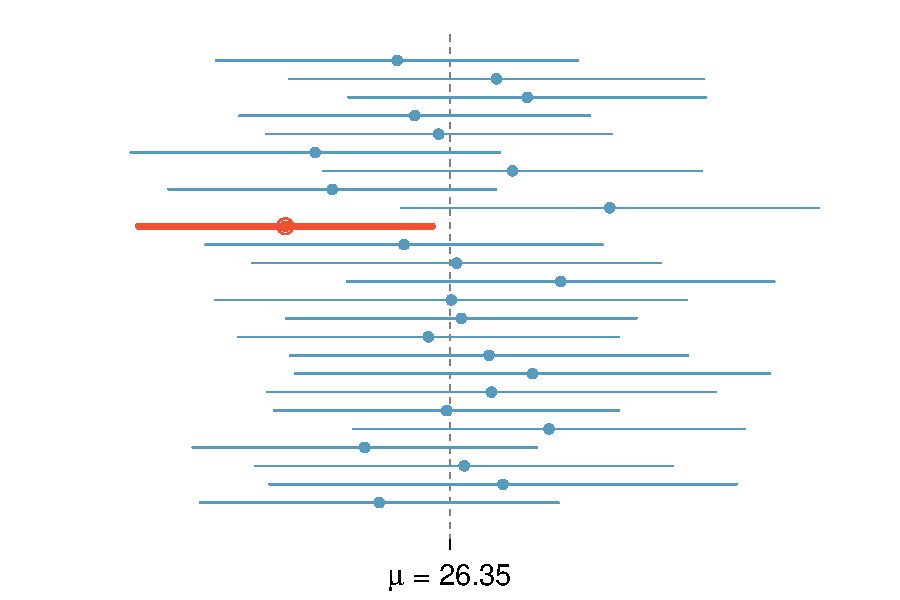
\includegraphics[width=\textwidth]{ch_inference_foundations_oi_biostat/figures/95PercentConfidenceInterval/95PercentConfidenceInterval}
   \caption{Twenty-five samples of size $n=100$ were taken from the \data{BRFSS} data set. For each sample, a 95\% confidence interval was created to try to capture the average adult BMI for the population. Only~1 of these~25 intervals did not capture the true mean.}
   \label{95PercentConfidenceInterval}
\end{figure}

\subsection{An approximate 95\% confidence interval through computation}
\label{95confidence}

A confidence interval contains information about a point estimate and the sampling variation. It can be completely defined by two attributes: its center and its width. The interval is centered at the best guess for where the population parameter is -- the point estimate -- and its width depends on how confident researchers are and the sampling variation of the point estimate. 

Roughly 95\% of the time, the estimate that is observed from resampling will be within approximately 2 standard errors of the population parameter. Equation ~\ref{95PercentConfidenceIntervalFormula}, introduced in Section ~\ref{mechanicsofInference}, allows scientists to be roughly \term{95\% confident} that the confidence interval has captured the population parameter:
\begin{eqnarray}
\text{point estimate}\ \pm\ 2 \times SE 
\label{95PercentConfidenceIntervalFormula}
\end{eqnarray}

The equation's components can be broken down into three parts: center, confidence level and standard error. These three parts can be understood mathematically or through repeated sampling.

A 95\% confidence interval computed through repeated sampling motivates the calculation of the confidence interval width: $2 \times SE$. How is the 95\% confidence interval estimated through \textsf{R}? Figure~\ref{brfssBMISamplingDistribution} should be inspiration on how to find a range of values that intends to capture the population parameter. 

As the mean of the sampling distribution is the mean of the population, building a 95\% confidence interval around an approximation of the sampling distribution is extremely reasonable. The sampling distribution represents all the possible values for an observed sample mean, so using the middle 95\% of the sampling distribution serves as a reasonable estimation for a 95\% confidence interval. \footnote{Ask Dave about this reasoning: why need to take 95\% values around the population parameter since we know that the mean is at the population mean? Sure there's variability but to be 95\% CI, 95\% chance of catching the population mean but through this computation, we know 100\% that it will always catch it if we take the middle 95\% of values}

Below is the pseudocode that implements this procedure using samples of size 40 \footnote{This highly resembles the pseudocode for approximating a sampling distribution from Section ~\ref{sampDist}}
\begin{verbatim}
(1) Create a vector to store the sample mean values once calculated 
(2) Take a sample of 40 from the BRFSS dataset
(3) Calculate the sample mean and store the value in (1)
(4) Repeat (2) and (3) many many times 
(5) Use the middle 95% of values as the 95% confidence interval. 
\end{verbatim}

The 95\% confidence interval through computation is the BMI value  $\mathrm{bmi}_1$ such that 2.5\% of the  values in the vector from Step 1 \footnote{denoted \var{sample.means} from Section ~\ref{seOfTheMean}} is below $\mathrm{bmi}_1$ and another BMI value $\mathrm{bmi}_2$ such that 2.5\% of the distribution is greater than $\mathrm{bmi}_2$

Recall from the distributions unit ~\ref{distributions}, to find these values, use the \var{quantile()} function in \textsf{R}. Particularly use the \var{quantile()} function on \var{sample.means}, the vector that that stores the sample means. 
\begin{verbatim}
confidence.interval<-quantile(x=sample.means,c(0.025,0.975))
> confidence.interval
    2.5%    97.5% 
24.79 	28.08
\end{verbatim}
The interval (24.79,28.08) is an estimation of a 95\% confidence interval using the sampling distribution of sample means. Scientists at the CDC are 95\% confident that the adult population mean BMI is between 24.79 and 28.08. Similarly if they calculated many confidence intervals from many different observed samples, 95\% of the confidence intervals that were calculated capture the population mean. 

\begin{exercise}
The CDC is interested in creating a 90\% confidence interval and a 50\% confidence interval. (a) how do the widths of the confidence intervals compare? (b) How would the \var{quantile()} function be used to find the 90\% and 50\% confidence intervals from using the vector \var{sample.means}?
 \footnote{(a) The 50\% confidence interval has the smaller width. In general the more confidence people want, the larger the confidence interval width will be.(b) Remember to grab the middle percent of observed sample means. The \textsf{R} code for calculating a 90\% confidence interval is \var{quantile(x=sample.means,c(0.05,0.95))}. For a 50\% confidence interval, the code would be \var{quantile(x=sample.means,c(0.25,0.75))}}
\end{exercise}

However, the CDC would not calculate a 95\% confidence interval through repeated sampling in \textsf{R}. The CDC does not have access to the entire US population, and it cannot resample the US population independently 100,000 times. Even more, it can never observe the sampling distribution. Yet, this procedure is useful to capture the essence of confidence intervals: incorporating variability. 


\subsection{Calculating an approximate 95\% confidence interval}
\label{calculate95confidence}

Only observing one sample mean, the CDC uses Equation ~\ref{95PercentConfidenceIntervalFormula} instead. With the goal of capturing the population parameter, the confidence interval is centered around where the population parameter is believed to be -- the sample mean. 

Section ~\ref{95confidence} indicates that the width of the interval depends on the confidence level as well as variance of the sampling distribution. For a given confidence level, a sampling distribution with high variance results in a wider confidence interval than one with low variance. The confidence level width must encompass uncertainty from the confidence level and randomness from sampling variability. Recall from Section \ref{seOfTheMean} the definition standard error. Standard error again becomes a natural measurement of uncertainty for building the interval.  

Roughly 95\% of the time, the estimate that is observed from resampling will be within approximately 2 standard errors\footnote{1.96 to be more precise if the sampling distribution resembles a Normal Distribution. Details coming up in Section ~\ref{sampdistmean}} of the population parameter. To be 95\% confident an interval will capture the population parameter, the confidence interval is two standard errors wide on each side. 

The three parts -- center, confidence level and standard error -- in Equation ~\ref{95PercentConfidenceIntervalFormula} allow scientists to include sampling variability in their estimates and be roughly \term{95\% confident} that the confidence interval has captured the population parameter from the sample observed. 

The 95\% confidence interval calculated from the \data{BRFSS BMI} sample with an observed sample mean of 26.53 and sample standard deviation of 5.84 is
\begin{align*}
\text{point estimate}\ &\pm\ 2 \times SE\\
26.53 &\pm 2\times \frac{5.84}{\sqrt{40}}\\
26.53 &\pm  1.85\\
(24.68 &, 28.38)
\end{align*}
While not exact, the confidence interval simulated through \textsf{R}  achieves a very similar confidence interval to the one through calculation. The difference is due to randomness in center and standard error of the single \data{BRFSS BMI} sample observed. 

\begin{exercise}
How does the center of the confidence interval from the \data{BRFSS BMI} sample differ from the center of the confidence interval computed in Section ~\ref{95confidence}? \footnote{The confidence interval computed in \textsf{R} is exactly the population mean. The center of the confidence interval from the \data{BRFSS BMI} sample is what the CDC believes to be the best guess for the population mean. Because the CDC only observes one sample, the center of the confidence interval will most likely be not equal to the population parameter due to sampling variation. }
\end{exercise}

\begin{exercise}
In Figure~\ref{95PercentConfidenceInterval}, one interval does not contain a BMI value of $\mu$. Does this imply that the average population BMI cannot be $\mu$? \footnote{Just as some observations occur more than two standard deviations from the mean, some point estimates will be more than two standard errors from the parameter. A confidence interval only provides a plausible range of values for a parameter. While other values are implausible based on the data, this does not mean they are absolutely impossible.}
\end{exercise}

The statement "about 95\% of observations are within two standard deviations of the mean" is only approximately true. This rule of thumb holds very well if the sample means are distributed normally. As Section ~\ref{cltSection} soon shows, the sample mean tends to be normally distributed when the sample size is sufficiently large. 

\begin{example}{The CDC is interesting in how the average heights of men and women differ. The scientists create 95\% confidence intervals for the average male height and the average female height from samples taken from the \data{BRFSS} dataset. With 40 men and 40 women, the average male height is 67.05 inches and the average female height is 66.50 inches. The sample standard deviations for males and females  are 3.82 and 4.14 respectively. What are the 95\% confidence intervals for the average male and female height in the US? }
\label{CIforGenderHeight}
Both 95\% confidence intervals are calculated using the formula \[\text{point estimate}\ \pm\ 2 \times SE\] and the information given above: 
\begin{align*}
\text{men: }\overline{\mathrm{age}_\mathrm{men}} &\pm\ 2 \times SE\\
67.05 &\pm 2\times \frac{3.82}{\sqrt{40}}\\
(65.84 &, 68.26)
\end{align*}
\begin{align*}
\text{women: }\overline{\mathrm{age}_\mathrm{men}}\ &\pm\ 2 \times SE\\
66.50 &\pm 2\times \frac{4.14}{\sqrt{40}}\\
(65.19 &, 67.81)
\end{align*}
The confidence intervals for average height by gender are different. It appears that the average heights are slightly different by gender but the CDC cannot formally conclude this. Chapter ~\ref{inferenceForNumericalData} will introduce how to compare the average heights of men and female directly. 
\end{example}

The 95\% confidence interval depends largely on the center and the standard error. Section ~\ref{changingTheConfidenceLevelSection} will explore how the multiplier changes beyond two standard errors as confidence levels change. 

\begin{exercise} \label{95CIExerciseForBRFSSAge}
The sample data \data{BRFSS BMI} suggests the average adult's age is about 48.85 years with a standard error of 2.95 years (estimated using the sample standard deviation, 18.69). What is an approximate 95\% confidence interval for the average age of US adults?\footnote{Again apply Equation~(\ref{95PercentConfidenceIntervalFormula}): $48.85 \ \pm \ 2\times 2.95 \rightarrow (42.95, 54.75)$. The interpretation of the interval is, "We are about 95\% confident the average age of US adults is between 42.95 and 54.75 years." Looking at the entire \data{BRFSS} dataset that the \data{BRFSS BMI} sample is drawn from (normally scientists do not have this luxury!), the average age is 46.72 which is indeed within the confidence interval just calculated.}
\end{exercise}

\subsection{The sample size for a sampling distribution}
\label{sampdistmean}

Figure~\ref{brfssBMISamplingDistribution} introduced the sampling distributions for $\overline{\mathrm{bmi}}$ of size 5 and 40. The sampling distribution for $n=5$ in Figure ~\ref{sampleMeanPrecision} was slightly skewed but more symmetric for $n=40$ . Figure \~ref{sampDistNormal} is a histogram of the sample means for 100,000 different random samples of size $n=40$ with a normal probability plot of those sample means. 

\begin{figure}[hht]
   \centering
   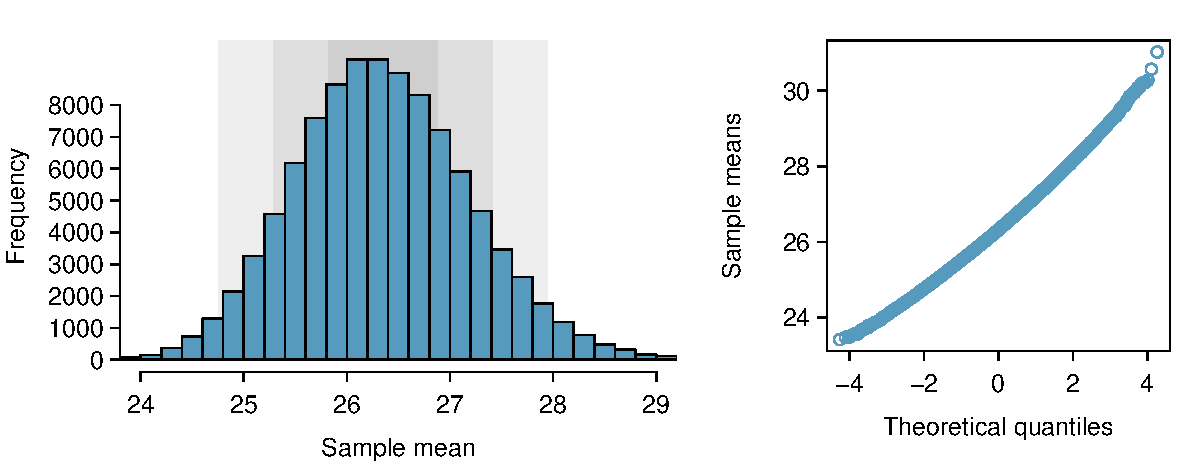
\includegraphics[width=\textwidth]{ch_inference_foundations_oi_biostat/figures/sampDistNormal/sampDistNormal}
   \caption{The left panel shows a histogram of the sample means for 100,000 different random samples of size $n=40$. The right panel shows a normal probability plot of those sample means.}
   \label{sampDistNormal}
\end{figure}

Does this sampling distribution resemble a familiar probability distribution (think back to Chapter ~\ref{modeling})? Hopefully so! The sampling distribution of sample means closely resembles the normal distribution (see Section~\ref{normalDist}). The right panel of  Figure~\ref{sampDistNormal} is a normal probability plot to evaluate if the sample means are approximately normally distributed. Because all of the points closely fall around a straight line, the distribution of sample means is nearly normal. This result can be explained by the Central Limit Theorem\footnote{A more formal definition coming soon in ~\ref{cltSection}}.

\begin{termBox}{\tBoxTitle{Central Limit Theorem, informal description}
If a sample consists of at least 30 independent observations and the data are not strongly skewed, then the distribution of the sample mean is well approximated by a~normal model.\index{Central Limit Theorem}}
\end{termBox}


\subsubsection{Why 30?}
\label{why30}

This text offers a cutoff at 30 for the sample size under the Central Limit Theorem but this rule of thumb varies from book to book. Using \textsf{R}, how could this rule of thumb be tested with the \data{BRFSS} data? Is 30 independent observations for the sample size a sufficient number to approximate the sampling distribution of the sample mean to a normal model? 

To test this, values below 30 should be considered as alternative sample sizes. The sampling distribution should be compared to a normal distribution for fit, and overlaying a normal approximation onto the sampling distribution histogram in \textsf{R} is an effective way to make such a comparison.  \footnote{Use the same code for creating a sampling distribution but vary the sample size. Then use the code: 
\var{hist(sample.means, freq=FALSE ) \\
curve(dnorm(x,mean=mean(sample.means), sd=sqrt(var(sample.means))), add = TRUE)} where the function \var{curve()} adds the normal curve on top of the histogram with parameters \var{mean(sample.means)} and \var{var(sample.means)} for the mean and the variance of the normal distribution.}

Figure ~\ref{cltThirty} displays the sampling distributions of the sample mean for sample sizes of 5, 10, 20 and 30. The overlaying curve on each histogram is a normal density curve with the normal distribution $\mathcal{N}(\mu, \sigma)$ where $\mu$ is the mean of the sample means and $\sigma$ is the standard deviation of the sample means.

\begin{figure}[hht] 
   \centering
   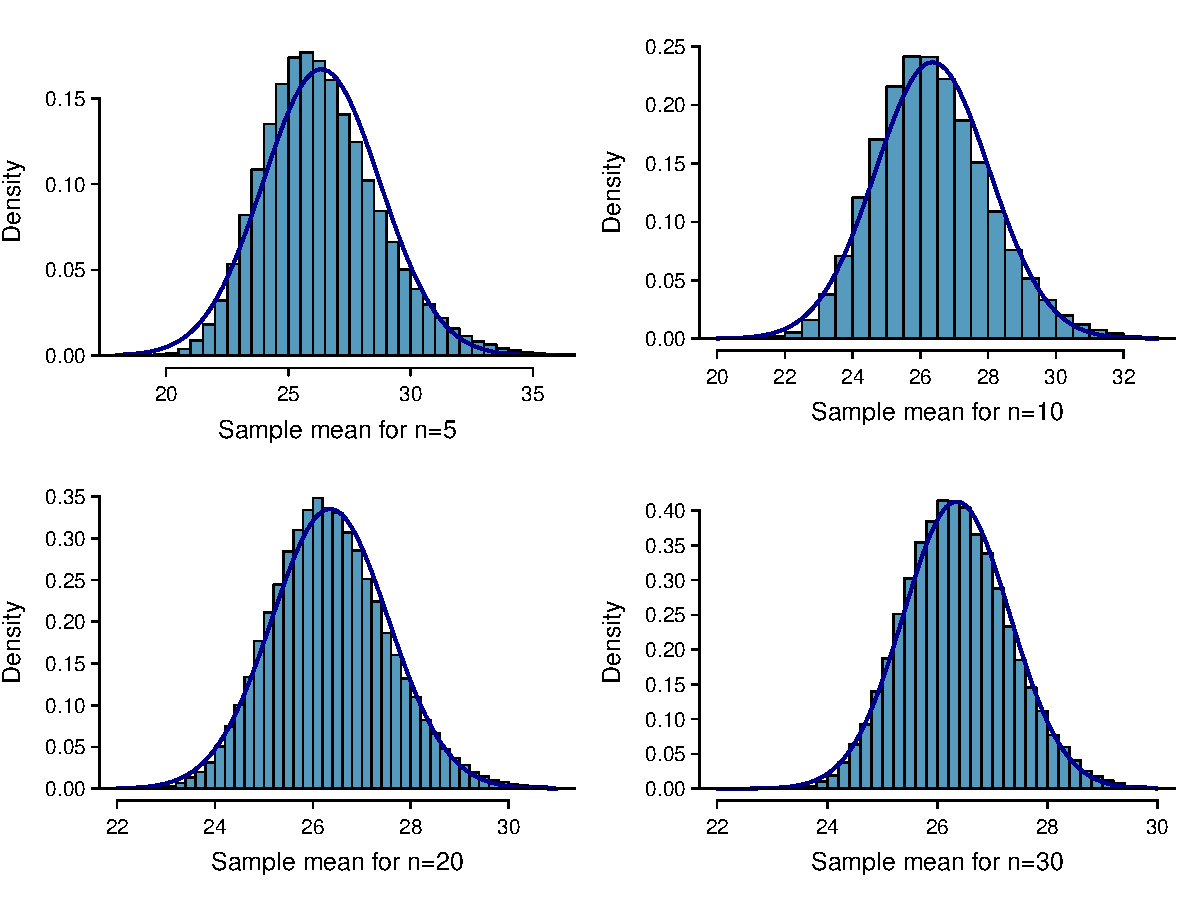
\includegraphics[width=\textwidth]{ch_inference_foundations_oi_biostat/figures/clt30/clt30}
   \label{cltThirty}
   \caption{The sampling distribution of sample means with different sample sizes $n=5, 10, 20, 30$. With a normal density curve superimposed, a normal model begins to become a fitting approximation for $n=30$, confirming the Central Limit Theorem rule of thumb.}
\end{figure}
\footnote{Ask Dave: is n=30 obviously better i.e. look at the curves and how they intersect the corners}

Using two standard errors in Equation~(\ref{95PercentConfidenceIntervalFormula}) indicates that roughly 95\% of the time, observations are within two standard deviations of the mean. Under the normal model, with a sufficient number of samples ($n\geq 30$), the equation is more precise using 1.96 in place of 2.
\begin{eqnarray}
\text{point estimate}\ \pm\ 1.96\times SE
\label{95PercentCIWhenUsingNormalModel}
\end{eqnarray}
If the distribution of the point estimate, such as $\overline{x}$, follows a normal model with standard error $SE$, Equation ~\ref{95PercentCIWhenUsingNormalModel} is used to create a 95\% confidence interval 

\subsection{Changing the confidence level}
\label{changingTheConfidenceLevelSection}

\index{confidence interval!confidence level|(}

Scientists generally build confidence intervals at 95\% confidence but depending on the application, the level may differ. Measuring the average BMI for US adults is a fairly low risk problem if the population parameter were measured incorrectly so the CDC might opt for a lower confidence. Instead consider the US Food and Drug Administration (FDA) studying a drug's effect on children. In this context, evidence at the 99\% confidence level may be more preferred as making a Type I Error is more costly.   

Parameters of more critical problems can call for a higher confidence levels in calculating confidence intervals and performing hypothesis tests \footnote{In many cases, these are not the only factors that determine a confidence level. Funding, logistics, and the number of observations that will be taken are all considered when choosing a confidence level}.

Think back to the analogy of catching a fish: if fishermen want to be more sure of catching fish, they use a wider net. To be more than 95\% confidence the population parameter is within the confidence interval, the interval must have larger widths. If they want an interval with lower confidence, such as 90\%, they would make the 95\% confidence interval slimmer.

The structure of the 95\% confidence interval in Equation ~\ref{95PercentCIWhenUsingNormalModel} resembles the equation to create intervals of different confidence levels. Recall from Section \label{calculate95confidence} that a confidence interval is defined by its center and width. The width, not center, changes with different confidence levels. Within a normal distribution, 95\% of the area underneath a normal curve lies within 1.96 standard deviations from the center as seen in Figure ~\ref{choosingZForCI}. 

\begin{exercise} \label{leadInForMakingA99PercentCIExercise}
If $X$ is a normally distributed random variable, how often will $X$ be within 2.58 standard deviations of the mean?\footnote{This is equivalent to asking how often the $Z$ score will be larger than -2.58 but less than 2.58. (For a visualization, see Figure~\ref{choosingZForCI}.) To determine this probability, look up -2.58 and 2.58 in the normal probability table (0.0049 and 0.9951). There is a $0.9951-0.0049 \approx 0.99$ probability that the unobserved random variable $X$ will be within 2.58 standard deviations of $\mu$.}
\end{exercise}

\begin{figure}
\centering
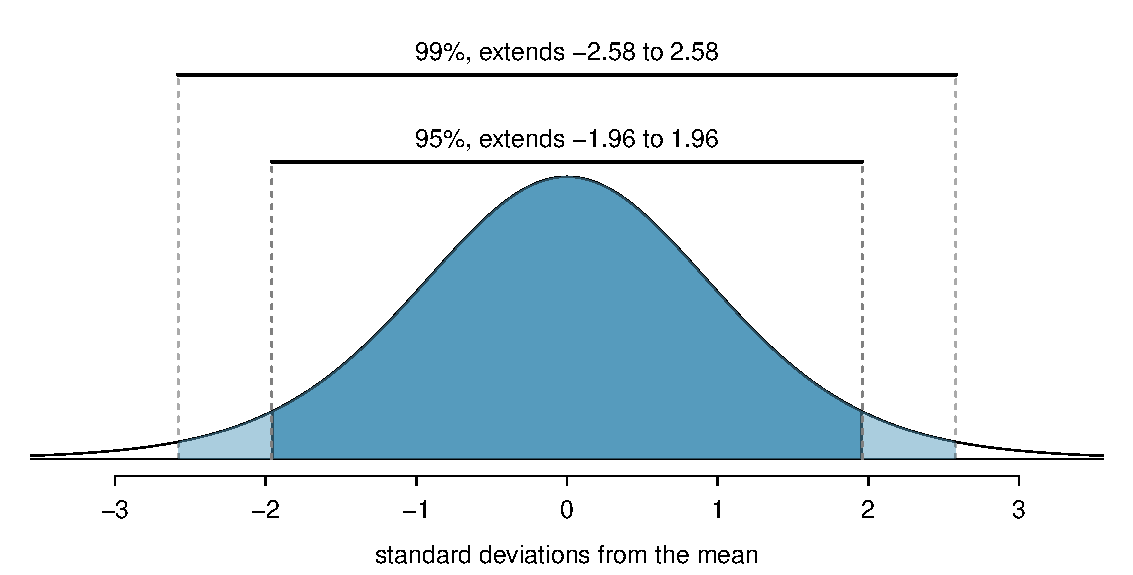
\includegraphics[width=\textwidth]{ch_inference_foundations_oi_biostat/figures/choosingZForCI/choosingZForCI}
\caption{If the confidence level is 99\%, choose $z^{\star}$ such that 99\% of the normal curve is between -$z^{\star}$ and $z^{\star}$, which corresponds to 0.5\% in the lower tail and 0.5\% in the upper tail: $z^{\star}=2.58$.}
\label{choosingZForCI}
\index{confidence interval!confidence level|)}
\end{figure}

The width of a 95\% confidence interval, $1.96\times SE$, and the computation example  in Section ~\ref{95confidence} reflect this relationship. The bounds of the 95\% confidence interval coincide with 1.96 times the standard deviation of the sampling distribution in the computation example given in Section ~\ref{95confidence}. 

The confidence level does not affect the standard error of the sampling distribution and cannot change the sample observed. It can only affect the multiplier, the "1.96," in calculating the width of the confidence interval. To calculate a 99\% confidence interval, the multiplier should instead be $2.58$, corresponding to the Z score of a normal distribution from Exercise~\ref{leadInForMakingA99PercentCIExercise}. 

This approach -- using the Z scores in the normal model to compute the multiplier for confidence levels -- is appropriate when $\overline{x}$ is distributed normally with mean $\mu$ and standard deviation $SE_{\overline{x}}$. The formula for a 99\% confidence interval of the population mean is 
\begin{eqnarray}
\overline{x}\ \pm\ 2.58\times SE_{\overline{x}}
\label{99PercCIForMean}
\end{eqnarray}

Equation ~\ref{99PercCIForMean} is not population mean specific. In fact, it can be generalized for any population parameter as \[\text{point estimate} \pm 2.58\times SE\]

The normal approximation is crucial for the precision of these confidence intervals. Section~\ref{cltSection} provides a more detailed discussion for when the normal model can safely be applied under the Central Limit Theorem. When the normal model is not a good fit, alternative distributions can be used that better characterize the sampling distribution. Below however is a good checklist to determine whether or not the Central Limit Theorem can be informally applied to the distribution of sample mean, and the Z score used as a multiplier for confidence interval.

\begin{termBox}{\tBoxTitle{Conditions for $\overline{x}$ being nearly normal and $SE$ being accurate\label{terBoxOfCondForXBarBeingNearlyNormalAndSEBeingAccurate}}
Important conditions to help ensure the sampling distribution of $\overline{x}$ is nearly normal and the estimate of SE sufficiently accurate:
\begin{itemize}
\setlength{\itemsep}{0mm}
\item The sample observations are independent.
\item The sample size is large: $n\geq30$ is a good rule of thumb.
\item The population distribution is not strongly skewed. (Check this using the sample distribution as an estimate of the population distribution.)
\end{itemize}
Additionally, the larger the sample size, the more lenient scientists are with the sample's skew.}
\end{termBox}

These three conditions help ensure that $\overline{x}$ is both distributed normally and representative of the target population. If the distribution of $\overline{x}$ is nearly normal, choosing a precise "1.96" or "2.58" becomes much easier for calculating confidence intervals. More importantly, however, the representativeness of the sample is imperative in the ability to infer about the target population. Randomness, independence and a large sample size safeguard against extreme observations skewing the sample. These conditions ensure the ability to accurately infer and generalize to the population of interest.

Verifying independence is often the most difficult of the conditions to check, and the way to check for independence varies from one situation to another. However, randomness is almost always necessary for independence. 

\begin{tipBox}{\tipBoxTitle{How to verify sample observations are independent}
Observations in a simple random sample consisting of less than 10\% of the population are independent.}
\end{tipBox}

\begin{caution}
{Independence for random processes and experiments}
{If a sample is from a random process or experiment, it is important to verify the observations from the process or subjects in the experiment are nearly independent and maintain their independence throughout the process or experiment. Usually subjects are considered independent if they undergo random assignment in an experiment or are selected randomly for some process.}
\end{caution}

\begin{exercise} \label{find99CIForBRFSSWeightExercise}
Create a 99\% confidence interval for the average male adult weight using the sample from Example ~\ref{CIforGenderHeight} The point estimate is $\overline{w_{\mathrm{men}}} = 172.65$ pounds and the standard error is $SE_{\overline{w_{\mathrm{men}}}} = 6.50$ pounds. Refer to Figure ~\ref{brfssMenWeight} for guidance on skewness.\footnote{The observations are independent (simple random sample, $<10\%$ of the population), the sample size is at least 30 ($n=403$), and the distribution is slightly skewed (Figure~\ref{brfssMenWeight}); the normal approximation and estimate of SE should be reasonable as only the skewness assumption is weakly not satisfied.  Apply the 99\% confidence interval formula: $\overline{w_{\mathrm{men}}}\ \pm\ 2.58 \times  SE_{\overline{w_{\mathrm{men}}}} \rightarrow (155.87, 189.43)$. There is 99\% confidence that the average weight of all US adult males is between 155.87 and 189.43 pounds.}
\end{exercise}

\begin{figure}
\centering
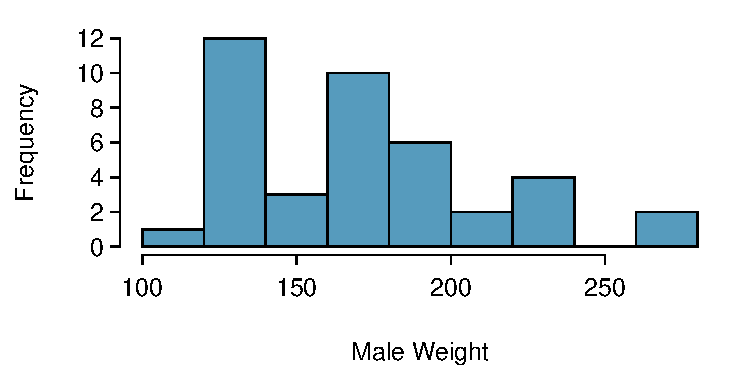
\includegraphics[width=\textwidth]{ch_inference_foundations_oi_biostat/figures/brfssMenWeight/brfssMenWeight.pdf}
\caption{The histogram of men's weights in the \data{BRFSS BMI} sample. There are 40 men in \data{BRFSS BMI}, and the weights are slightly skewed. With a sufficiently large sample size taken from a random sample, the sample mean can be considered nearly normal.}
\label{brfssMenWeight}
\index{confidence interval!confidence level|)}
\end{figure}

The calculation of a confidence interval for any confidence level can be generalized from the 95\% and 99\% confidence intervals. While it has become tradition to use the 95\% confidence level, confidence levels can vary by statistician, context and inference goal. 

\begin{termBox}{\tBoxTitle{Confidence interval for any confidence level (nearly normal model)}
If the point estimate follows the normal model with standard error $SE$, then a confidence interval for the population parameter is
\begin{eqnarray*}
\text{point estimate}\ \pm\ z^{\star} SE
\end{eqnarray*}
where the value of $z^{\star}$ corresponds to the confidence level selected. The coefficient on the standard error, $z^{\star}$, is also known as the critical value. $z^{\star}$ is only used when the point estimate resembles a normal model \footnote{$z^{\star}$ is also used when the population standard deviation is known. However this is rarely ever the case in practice as previously mentioned. This texts disregards this situation completely.}}
\end{termBox}
\begin{termBox}{\tBoxTitle{Margin of error}
\label{marginOfErrorTermBox}In a confidence interval, $z^{\star}\times SE$ is called the \term{margin of error} and is half the width of the confidence interval.}
\end{termBox}

Figure ~\ref{choosingZForCI} provides a picture of how to identify $z^{\star}$ based on a confidence level. Select $z^{\star}$ so that the area between -$z^{\star}$ and $z^{\star}$ in the normal model corresponds to the confidence level. Because $z^{\star}$ follows a standard normal distribution, $\mathcal{N}(0,1)$, scientists either use \textsf{R} software or a Z-table \footnote{also known as a Normal table} to find the critical value. The \var{qnorm()} function in \textsf{R} has probability $p$ as an input and outputs the quantile value $z$ such that $P(Z\leq z)=p$. For a 95\% confidence interval, $p=0.025$ as the confidence interval grabs the \emph{middle} 95\% of values. To find $z^{\star}$ in \textsf{R}\begin{verbatim}
> qnorm(0.025)
[1] -1.959964
\end{verbatim}
$z^{\star}=1.96$ is the critical value for 95\% \footnote{It does not matter if $z^{\star}$ is positive or negative since the half widths are on both sides of the point estimate.}. 
\begin{exercise} 
What is the critical value associated with (a) 90\%, (b) 75\% and (c) 50\%? \footnote{Remember to only consider the \emph{middle} values, and for any given confidence level $C$, type \var{qnorm($0.5\cdot (1-C)$)} into \textsf{R}.(a) \var{qnorm(0.05)= -1.644854} so $z^{\star}=1.65$ for a 90\% confidence level (b) 1.15 (c) 0.67}
\end{exercise}

\begin{exercise} \label{find90CIForBRFSSWeightExercise}
Use the data in Exercise~\ref{find99CIForBRFSSWeightExercise} to create a 90\% confidence interval for the average weight of men in the United States.\footnote{First find $z^{\star}$ such that 90\% of the distribution falls between -$z^{\star}$ and $z^{\star}$ in the standard normal model, $N(\mu=0, \sigma=1)$: $z^{\star}=1.65$. The 90\% confidence interval can then be computed as $\overline{w_\mathrm{men}}\ \pm\ 1.65\times SE_{\overline{w_\mathrm{men}}} \to (178.32, 199.78)$.  (The conditions for normality and the standard error were verified in in Exercise ~\ref{find99CIForBRFSSWeightExercise}.) That is, we are 90\% confident the average weight of males is between 178.32 and 199.78 pounds. Also note that because this confidence interval is at the 90\% confidence level, the interval width is smaller than that of Exercise ~\ref{find99CIForBRFSSWeightExercise}.}
\end{exercise}

\subsection{Interpreting confidence intervals}
\label{interpretingCIs}

\index{confidence interval!interpretation|(}

A careful eye might have observed the somewhat awkward language used to describe confidence intervals. Correct interpretation:
\begin{quote}
We are XX\% confident that the population parameter is between...
\end{quote}

Looking back to ~\ref{confidenceLevels}, a confidence level is defined as if a random sample from the population was drawn 100 times independently and a confidence interval was calculated around the point estimate each time, approximately 95 confidence intervals would contain the population parameter. 

Researchers in practice would almost never be able to resample 100 times and generate 100 confidence intervals. The meaning of being "95\% confident" has traditionally been one grounded in theory and less in practice. "Confidence" relates more to the reliability of the process of creating such a range and less so in the probability that the value is captured within the range. 

\emph{Incorrect} language might try to describe the confidence interval as capturing the population parameter with a certain probability. This is one of the most common errors: while it might be useful to think of it as a probability, the confidence level only quantifies how plausible the parameter is in the interval. 

Another especially important consideration of confidence intervals is that confidence intervals \emph{only try to capture the population parameter}. Intervals say nothing about the confidence of capturing individual observations, a proportion of the observations, a percent of all the data or just the sampled data. A confidence interval also deals nothing with capturing point estimates since it is always centered at the observed point estimate. Confidence intervals only attempt to capture and infer on population parameters.

Some incorrect interpretations of a 95\% confidence interval include: 
\begin{quote}
95\% of the observed data is between ...\\
95\% of the population distribution is contained in the confidence interval.\\
\end{quote}

Remember, a confidence interval is not a range of plausible values for the sample mean. The sample mean is already known. It is already observed. The confidence interval may be understood as an estimate of plausible values for the population parameter.

The differences in correct and incorrect interpretations are extremely nuanced. However the goal of this book is to provide the tools to calculate a confidence interval from data. The technical and precise wording of the interpretation of confidence intervals has little bearing in practice. 

\index{confidence interval!interpretation|)}
\index{confidence interval|)}

\subsection[Nearly normal population with known SD (special topic)]{Nearly normal population with known SD (special topic)}
\label{nearlyNormalPopWithKnownSD}

\index{Central Limit Theorem!normal data|(}

In rare circumstances important characteristics of a population are known. For instance, a population is already known to be nearly normal, and scientists do not need to rely on a rule of thumb of $n\geq 30$. Scientists might also know certain parameter values. Even so, a random sample still will be drawn to study other characteristics of the population. Consider the assumptions required to model the sample mean after a normal distribution: 
\begin{enumerate}
\setlength{\itemsep}{0mm}
\item[(1)] The observations are independent.
\item[(2)] The sample size $n$ is at least 30.
\item[(3)] The data distribution is not strongly skewed.
\end{enumerate}
These conditions are required to ensure the distribution of sample means is nearly normal. However, if the population is known to be nearly normal, the sample mean is always distributed normally (this is a special case of the Central Limit Theorem). If the population standard deviation is also known, then conditions (2) and (3) are not necessary for those data. 
\begin{example}{The heights of male seniors in high school closely follow a normal distribution $N(\mu=70.43, \sigma=2.73)$, where the units are inches.\footnote{These values were computed using the USDA Food Commodity Intake Database.} If the heights of five male seniors are randomly sampled, what distribution should the sample mean follow?}\label{simpleSampleOfFiveMaleSeniors}
The population, high school male seniors, is nearly normal, the population standard deviation is known, and the observations are from a random sample from a much larger population. These observations are considered independent. Therefore the sample mean is distributed normally with mean $\mu=70.43$ inches and standard error $SE=\sigma/\sqrt{n} = 2.73/\sqrt{5}=1.22$ inches.
\end{example}

\begin{termBox}{\tBoxTitle{Alternative conditions for applying the normal distribution to model the sample mean}
If the population is known to be nearly normal with a known population standard deviation $\sigma$, the sample mean $\overline{x}$ follows a nearly normal distribution $N(\mu, \sigma/\sqrt{n})$ if the sampled observations are independent. There is no uncertainty surrounding the standard deviation of population, and the point estimate for the population standard deviation, $s$, is meaningless in this context. The standard error calculated for confidence intervals instead uses the known population standard deviation where $SE = \sigma/\sqrt{n}$}
\end{termBox}

\begin{tipBox}{\tipBoxTitle{Relaxing the nearly normal condition}
As the sample size becomes larger, it is reasonable to \emph{slowly} relax the nearly normal assumption on the data for dealing with small samples. By the time the sample size reaches 30, the data must show strong skew to continue to have concerns about the normality of the sampling distribution.}
\index{Central Limit Theorem!normal data|)}
\end{tipBox}

In practice, the population standard deviation is rarely know, but the Central Limit Theorem allows the distribution of the sampling distribution to be described more specifically from samples of large sample sizes. 

%__________________
\section{Hypothesis testing}
\label{hypothesisTesting}

\index{hypothesis testing|(}

Beyond calculating a confidence interval, the CDC wants to see if the average US adult BMI has changed from 20 years ago. It wants to compare the average adult BMI in 2000 to that in 1980 ($\overline{\mathrm{BMI}}_{1980} =25.3$)\footnote{Flegal, KM, MD Carroll, RJ Kuczmarski, and CL Johnson. "Overweight and Obesity in the United States: Prevalence and Trends, 1960?1994." International Journal of Obesity (1998): 39-47. Web. \url{<http://www.ncbi.nlm.nih.gov/pubmed/9481598>}.}. The CDC is also concerned with the respiratory health of US coal miners. High levels of coal mine dust exposure increases the prevalence of coal workers' pneumoconiosis (black lung) and progressive massive fibrosis. In the 1992 \emph{American Industrial Hygiene Association Journal}, scientists collected data on dust exposure. With the Mine Safety and Health Administration (MSHA) permissible dust exposure limit of 2 $mg/m^3$, were coal mines adhering to this limit in 1992? 

Many questions like these, given the correct data, can be answered through hypothesis testing. \term{Hypothesis testing} is a method in statistics that evaluates whether or not a population parameter takes on some hypothesized value or not with an associated probability of error. This procedure, most obviously, determines the probability that a given hypothesis is true or not.

Hypotheses are often simple questions that have a yes or no answer. Consider some hypotheses below: \begin{quote}
Is the mean body temperature really $98.6^\circ$ F? \\
Has consumption of soda changed across the US overtime? \\
Do MCAT classes improve MCAT scores? 
\end{quote}

The hypothesis testing process consists of 5 steps. Going through the \term{hypothesis testing framework} allows scientists to answer these yes/no questions with a certain degree of confidence after observing a sample. This section begins by testing a hypothesis from observing a single sample. Hypothesis testing, as with confidence intervals, can help make inferences on two or more populations. Chapter ~\ref{foundationsForInference} only focuses on inference methods for the sample mean of a single population, but Chapter ~\ref{inferenceForNumericalData} expands further to two or more populations. 

Remember, hypothesis testing, as with confidence intervals, can concern any population parameter. The population mean, population standard deviation or even the population IQR all can be inferred using the correct inference methods.

\subsection{Hypothesis testing framework}
\label{hypothesisFramework}

The average BMI of \data{BRFSS BMI} is 26.53. The CDC wants to know if this sample provides enough evidence that adults are, on average, are healthy as they were 20 years ago versus the alternative, that they are not. This question can be simplified into two \termsub{hypotheses}: 
\begin{itemize}
\setlength{\itemsep}{0mm}
\item[$H_0$:] US adults in 2000 are on average as healthy as they were in 1980 with an average BMI of 25.3. 
\item[$H_A$:] The average US adult BMI in 2000 is not the same the average US adult BMI in 1980. 
\end{itemize}

\subsubsection{Step 1: Formulating hypotheses}

The first step within the hypothesis testing framework is setting up the hypotheses. As shown above, there are  generally two hypotheses, a null and an alternative. 

$H_0$ is called\marginpar[\raggedright\vspace{6mm}

$H_0$\\\footnotesize null hypothesis\vspace{3mm}\\\normalsize $H_A$\\\footnotesize alternative\\ hypothesis]{\raggedright\vspace{6mm}

$H_0$\\\footnotesize null hypothesis\vspace{3mm}\\\normalsize $H_A$\\\footnotesize alternative\\ hypothesis} the null hypothesis and $H_A$ the alternative hypothesis.

\begin{termBox}{\tBoxTitle{Null and alternative hypotheses}
{\small The \term{null hypothesis ($H_0$)} often represents either a skeptical perspective or a claim to be tested. The \term{alternative hypothesis ($H_A$)} represents an alternative claim under consideration and is often represented by a range of possible parameter values.}}
\end{termBox}

The null hypothesis often represents a skeptical position or a common view on something. The null hypothesis is generally denoted as "no difference" or what one would observe if there is no change.  The alternative hypothesis often represents a new perspective, such as the possibility that there has been a change or a new discovery. If the null hypothesis is true, any difference between the observed sample is due only to chance variation. 

\begin{tipBox}{\tipBoxTitle{Hypothesis testing framework}
The logic of hypothesis testing is that the null hypothesis ($H_0$) will not be rejected, unless the evidence in favor of the alternative hypothesis ($H_A$) is so strong that $H_0$ must be rejected in favor of $H_A$.}
\end{tipBox}

The framework's first step is used often beyond scientific research but describes the very nature of the scientific method. If a person makes a somewhat unbelievable claim, people are initially skeptical. The nulll hypothesis $H_0$ is generally believed unless there is sufficient observed evidence that does not support the claim. Then the null hypothesis is rejected in favor of the alternative. 

\begin{exercise} \label{hypTestStudyExample}
A new study would like to be published in a scientific journal. The board that determines the validity of the study considers two possible claims about this study: either the study is valid or it is pseudoscience. Using the hypothesis framework, which of these claims would be the null hypothesis and which the alternative? \footnote{The board begins as somewhat skeptical of the discovery. It considers whether the study's methodology, results and reproducibility is convincing enough for the study to be valid. If the study is legitimate, the board rejects the null hypothesis (The study is pseudoscience. There is no change.) and concludes the study is valid and should be published (the alternative hypothesis).}
\end{exercise}

Even if the board of the journal leave unconvinced that the study is publishable, these board members do not necessarily believe the study is a complete fabrication. Hypothesis testing is the same: \emph{even if the null hypothesis is not rejected, it cannot be accepted}. Failing to find strong evidence for the alternative hypothesis is not equivalent to accepting the null hypothesis. 

\begin{tipBox}{\tipBoxTitle{Double negatives can sometimes be used in statistics}
Many times in statistics, double negatives can be used. For instance, scientists might say that the null hypothesis is \emph{not implausible} or they \emph{failed to reject} the null hypothesis. Double negatives are used to communicate that while a position is not being rejected, it is also not accepted as truth.}
\end{tipBox}

The null hypothesis is, using the \data{BRFSS BMI} sample, the average US adult BMI in 2000 equals 25.3, the average in 1980. 

The alternative hypothesis represents something new or more interesting: the average US adult BMI has changed since 1980. These hypotheses can be described in mathematical notation using $\mu_{\mathrm{bmi}}$ as the average BMI for US adults in 2000.
\[H_0:\mu_{\mathrm{bmi}} = 25.3 \hspace{0.5in} H_A: \mu_{\mathrm{bmi}} \neq 25.3\]

Using this mathematical notation, the hypotheses can now be evaluated using statistical tools. In this context, 25.32 is referred to as the \term{null value} since it represents the value of the parameter if the null hypothesis is true. The \data{BRFSS BMI} sample will be used to evaluate these hypotheses. 

Note it is important to remember that the CDC is not testing whether or not the average BMI from \data{BRFFS BMI} is 25.3 or not. The CDC already observes all the values within \data{BRFSS BMI} and can simply calculate the average BMI. Rather these hypotheses are testing if the \emph{population parameter} of all US adults is 25.3 or not. 

\begin{tipBox}{\tipBoxTitle{Null and Alternative Hypothesis Setup}
The null hypothesis is generally written as $H_0: \mu=\mu_0$ where $\mu$ is the population mean and $\mu_0$ is the hypothesized value that is believed to be true.The alternative hypothesis, on the other hand, can have the population parameter take on many values. \\ 
The alternative hypothesis can take on many forms. If the researchers are interested in showing any difference --an increase or decrease-- then the safest alternative hypothesis choice would be $\mu\neq \mu_0$, a two-sided alternative. If there exist a prior belief of how $\mu$ and $\mu_0$ compare or researchers are interested in only showing an increase or decrease, not both, a one-sided alternative, $\mu\geq \mu_0$ or $\mu \leq \mu_0$ should be used. Section ~\ref{pValue} will go into more detail on one-side versus two sided alternative hypotheses.}
\end{tipBox}

\subsubsection{Step 2: Specifying a significance level $\alpha$}
After researchers stated a null and alternative hypothesis, they then need to specify a \term{significance level}. The significance level $\alpha$ is the acceptable error probability of the test. In hypothesis testing, the error probability is the probability of incorrectly concluding the alternative hypothesis is true when it is, in fact, not true. This error is called a Type I error, and $\alpha$ is the probability of making a Type I error. Section \ref{DecisionErrors} goes into more detail on error types. 

Typically, $\alpha$ is taken to be 0.05, 0.01, or some other small value. $\alpha$ plays the same role as the error probability in confidence intervals, and is a measure of uncertainty. If $\alpha=0.05$, the hypothesis test will be performed at a 95\% confidence level. Section ~\ref{utilizingOurCI} provides a clearer connection between hypothesis testing and confidence intervals.  

\subsubsection{Step 3: Calculating the test statistic}
The third step is calculating a test statistic from the observed data. The test statistic measures the difference between the observed point estimate and what is expected if the null hypothesis is true. It answers the question: "How many standard deviations from the null value is the observed sample value?" The test statistic is used in Step 4 and 5 to arrive at a conclusion. 

Thinking back to Section ~\ref{normalDist}, the test statistic follows a similar construction as standardizing a normal distribution. For hypothesis tests inferring on a population mean where the population standard deviation is unknown, the test statistic will always be 
\begin{eqnarray}T=\frac{\overline{x}-\mu_0}{s/\sqrt{n}}\end{eqnarray} 
where $\overline{x}$ is the sample mean, $s$ is the sample standard deviation and $n$ is the number of observations in the sample. 

\emph{Note:} In general, test statistics follow the form $\frac{\mathrm{observed-hypothesized}}{\text{standard error}}$ to calculate the number of standard deviations the observed value is from the hypothesized value. This T-statistic, $T$, follows a $t$-distribution and will have $n-1$ degrees of freedom. The $t$- distribution is covered more extensively in Section ~\ref{tdistribution}

\begin{termBox}{\tBoxTitle{Test statistic}
A \emph{test statistic} is a special summary statistic that is particularly useful for evaluating a hypothesis test. The test-statistic summarizes how many standard deviations the observed sample value is from the hypothesized null value and follows a $t$-distribution with $n-1$ degrees of freedom. The $t$-distribution will be covered in Section ~\ref{tdistribution} \footnote{When a point estimate is nearly normal, the Z score of the point estimate can be used as the test statistic. Later chapters will encounter situations where other test statistics are helpful.}}
\index{hypothesis testing!using normal model|)}
\end{termBox}

\subsubsection{Step 4: Calculating the p-value}
Consider a T-statistic of 10. This means that the observed sample mean is 10 standard deviations away from the hypothesized value under the null hypothesis. Observing the sample mean is such a rare event since it is so far away from the hypothesized value, but how rare is observing a value 10 standard deviations away from the mean? 10\% likely? 1\% likely? 0.001\%?

The \term{p-value} is the probability of observing a point estimate or a more extreme point estimate assuming the null hypothesis is true. The p-value allows the researchers to make conclusions from the T-statistic. Formally the p-value is a conditional probability.

\begin{termBox}{\tBoxTitle{p-value}
The \term{p-value}\index{hypothesis testing!p-value|textbf} is the probability of observing data at least as favorable as the current sample to the alternative hypothesis, if the null hypothesis is true. A summary statistic of the data is typically used to help compute the p-value and evaluate the hypotheses.}
\end{termBox}

How is this probability calculated? Section ~\ref{pValue} will go into more detail from using \textsf{R}, and the Z and $t$-tables. 

\subsubsection{Step 5: Making the conclusion}
The final step within the hypothesis testing framework is to make a conclusion.

A large T-statistic indicates an extreme observation, and the probability associated with observing an extreme point estimate will be small. A low p-value from Step 4 provides evidence that the null value is unlikely and results in a rejection of the null hypothesis. The smaller the p-value, the strong the evidence to against the null hypothesis. 

How small is small? The significance level, $\alpha$ from Step 2 determined whether or not scientists reject the null hypothesis. If the p-value is smaller than $\alpha$ (usually 0.01 or 0.05), the null hypothesis is rejected. The scientists conclude that the T-statistic and conclusion are statistically significant at the $\alpha$ level. 

If the p-value is $\alpha$ or greater, there is not enough evidence to reject the null hypothesis. Failure to reject $H_0$ is not equivalent to acceptance of $H_0$ (refer to Example \ref{hypTestStudyExample} for clarity). 

In practice, however, failure to reject $H_0$ is equivalent to accepting $H_0$, and rejecting $H_0$ is equivalent to accepting $H_A$. Most importantly, it is key that researchers state the conclusion in the context of the original problem, using the language and units of the inference question. Many times this is forgotten, but it is absolutely necessary in both theory and practice. 

\subsection{Calculating p-values}
\label{pValue}

\index{hypothesis testing!p-value|(}

Calculating p-values can be the most difficult part of the hypothesis testing framework. The p-value depends on many moving parts: the T-statistic, the sample size and the alternative hypothesis, but always remember, if the p-value is smaller than $\alpha$, the sample indicates that something rare was observed. So rare that the null hypothesis should be rejected as true. 

\begin{figure}[ht]
   \centering
   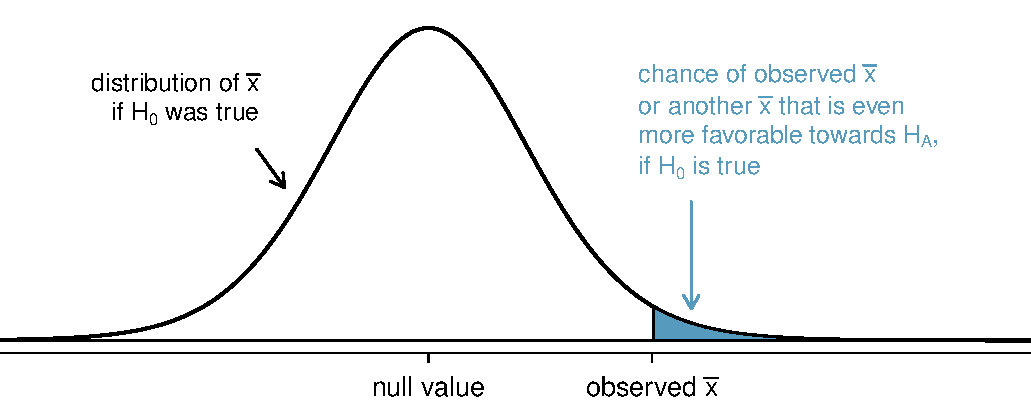
\includegraphics[width=0.9\textwidth]{ch_inference_foundations_oi_biostat/figures/pValueOneSidedSleepStudyExplained/pValueOneSidedSleepStudyExplained}
   \caption{To identify the p-value, the distribution of the sample mean under the null hypothesis is considered. The p-value is defined as the probability of observing the $\overline{x}$ or a sample mean even more extreme. The p-value implies whether or not it is favorable to follow $H_A$ under this distribution.} 
   \label{pValueOneSidedSleepStudyExplained}
\end{figure}

The shaded area in Figure~\ref{pValueOneSidedSleepStudyExplained} is the p-value for a one sided alternative $\mu > \mu_0$. If the alternative hypothesis is one sided and has the form $\mu > \mu_0$, then the p-value is the area of the shading the upper tail. If the alternative is one sided but has the form $\mu < \mu_0$, then the p-value would be the shaded area in the lower tail, left of the observed $\overline{x}$ wherever it may lie. If the alternative were $\mu < \mu_0$, the shaded area would be the majority of the distribution in Figure~\ref{pValueOneSidedSleepStudyExplained}. In a two-sided test, \emph{two tails are shaded} since evidence in either direction is favorable to $H_A$ (Figure ~\ref{2ndSchSleepHTExample}). 

\begin{figure}
   \centering
   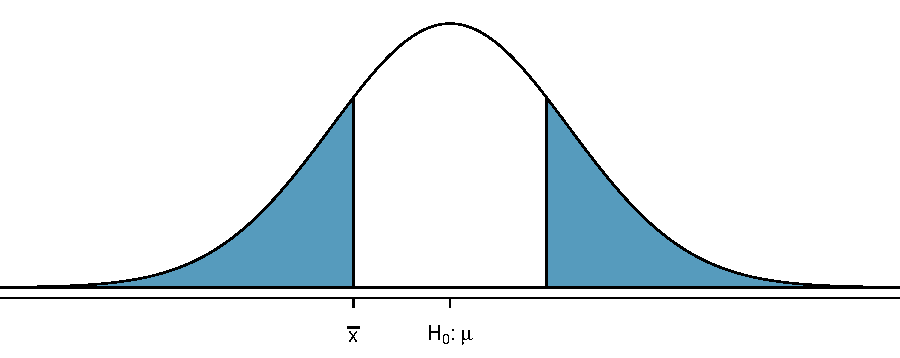
\includegraphics[width=0.9\textwidth]{ch_inference_foundations_oi_biostat/figures/2ndSchSleepHTExample/2ndSchSleepHTExample}
   \caption{$H_A$ is two-sided, so \emph{both} tails must be counted for the p-value. Observing a significance change -- increase or a decrease --  would be favorable to $H_A$.}
   \label{2ndSchSleepHTExample}
\end{figure}

How do scientists quantify this shaded area? The process of finding the p-value from a T-statistic is analogous to using a Z-score to find the shaded area underneath a normal curve. Recall the example where the CDC compares adult health in 2000 to adult health in 1980 with the following hypotheses: \[H_0:\mu_{\mathrm{bmi}} = 25.3 \hspace{0.5in} H_A: \mu_{\mathrm{bmi}} \neq 25.3\]

Consider a sample of 50 people with a sample mean of 24. The sample standard deviation is 5. The T-statistic is therefore \footnote{calculating the T-statistic using the sample mean from the \data{BRFSS BMI} dataset is an exercise in the book}. \[T=\frac{24-25.3}{5/\sqrt{50}}= -1.84\] The T-statistic is analogous to the Z-score (standard score) that indicates how many standard deviations the observed sample mean is from the null value. This standardization becomes a great way to unify all the moving parts in order to calculate the p-value. 

Step 3 concludes with the T-statistic as -1.84. Calculating the p-value in Step 4 begins with the distribution of the T-statistic. Recall from Section ~\ref{hypothesisFramework}, the T-statistic follows a $t$-distribution with $n-1$ degrees of freedom.  Section ~\ref{tdistribution} offers an introduction to the $t$-distribution, and if $n\geq 30$, the T-statistic can resemble a normal distribution. Scientists prefer to approximate the distribution of the T-statistic to a normal because of the attractive qualities introduced in Chapter ~\ref{modeling} that a normal distribution offers. 

Researchers can either use a Z or $t$-table to find the p-value, or in most cases, use \textsf{R} once the T-statistic and its distribution is known. When $n<30$, scientists use a $t$-table like the one in Appendix~\ref{tDistributionTable} on page~\pageref{tDistributionTable}. If $n\geq 30$, Z tables are used, found in Appendix ~\ref{normalProbabilityTable} on page ~\pageref{normalProbabilityTable}. The $t$-table lists the approximate area for one or two tailed alternative hypotheses whereas the Z table only indicates the area left of the T-statistic, coinciding with a one-sided alternative. However, because normal distributions are symmetric, finding the p-value for a two sided alternative is just the value from a Z table times two!

The T-statistic of -1.84 was calculated from a sample of 50 people. The Z table indicates that the area to the left of -1.84 is 0.0329. Because the alternative hypothesis is two-sided, $\mu_{\mathrm{bmi}} \neq 25.3$, the area shaded is similar to Figure ~\ref{2ndSchSleepHTExample}. Both tails are shaded. Therefore the p-value is 
\begin{align*}
p &=Pr(T\leq -1.84) + Pr(T\geq 1.84)\\
&= Pr(|T| \leq -1.84)\\
&= 2Pr(T\leq -1.84)\\
&= 2 \cdot 0.0329\\
&= 0.0658
\end{align*}

If the CDC did not want to use the rule of thumb, $n\geq 30$, they would use the $t$-table. A T-statistic of -1.84 and 49 ($n-1$) degrees of freedom result in a p-value between 0.1 and 0.05 for a two-sided alternative. The $t$-table lists fewer values than the Z-table so the resulting p-value is imprecise. 

If available, \textsf{R} is also a handy tool. Use the \var{pt()} or the \var{pnorm()} function to calculate the area left of the T-statistic. However be mindful that like in Figure ~\ref{pValueOneSidedSleepStudyExplained}, the area left of the T-statistic is not necessarily always the p-value. \footnote{Figure ~\ref{pValueOneSidedSleepStudyExplained} is the distribution of the sample mean, not the distribution of the T-statistic. The distribution of the T-statistic is very similar because the T-statistic is the sample mean normalized. It is centered at 0 (the null value in the sample distribution), and $\overline{x}$ is analogous to the T-statistic. The shaded area, therefore, remains the same.} The complement of the \textsf{R} output may need to be used to isolate the appropriate area of the distribution. 

The $n\geq 30$ threshold does not need to be followed when using \textsf{R} as the function \var{pt()} becomes just as easy and more accurate as approximating to a normal distribution. As $n$ increases, normal and $t$-distributions almost become equivalent, evidenced by Section ~ref{distribution}. 

Using \textsf{R}, \var{pnorm()} and \var{pt()} are both used to demonstrate. \begin{verbatim}
> 2*pnorm(-1.84)
[1] 0.06576824
> 2*pt(-1.84,49)
[1] 0.07182936
\end{verbatim}

\textsf{R} produced extremely similar outputs for the p-value. With a T-statistic of -1.84, the CDC determines through the Z-table and through \textsf{R} that the p-value is approximately 0.07. 

The CDC proceeds to Step 5 to make a conclusion in the context of the question. The p-value (0.07) is less than the significance level, $\alpha=0.05$, established in Step 2. $H_0$ can be rejected. In context, after observing a sample mean of 24 for the average BMI in the US in 2000, a p-value of 0.07 was observed. This p-value is less than 0.05. Therefore the average BMI from the observed sample suggests that the average adult population BMI is not 25.3, the average in 1980. There exists a noticeable difference between the health of adults from 1980 to 2000. 

\begin{termBox}{\tBoxTitle{p-value as a tool in hypothesis testing}
The p-value quantifies how strongly the data favor $H_A$ over $H_0$. A small p-value (usually $<0.05$) corresponds to sufficient evidence to reject $H_0$ in favor of $H_A$.}
\index{hypothesis testing!p-value|)}
\end{termBox}

\begin{exercise}
If the null hypothesis is true, how often should the p-value be less than 0.05?\footnote{About 5\% of the time. If the null hypothesis is true, then the data only has a 5\% chance of being in the 5\% of data most favorable to $H_A$.}
\index{data!school sleep|)}
\end{exercise}

\begin{tipBox}{\tipBoxTitle{Concluding from Critical Values}
Conclusions are made from the relationship between the p-value and the significance level, but if $\alpha$ is some common value like 0.05, the critical value can offer a quick shortcut to the conclusion. \\

Recall that critical value is the coefficient of the standard error in the confidence interval formula. The critical value is also the value on the normalized sampling distribution that can be compared to the T-statistic in hypothesis testing. If the absolute value of the T-statistic is greater than the critical value (the T-statistic is more extreme), the p-value is less than $\alpha$ and the null hypothesis can be rejected.}
\end{tipBox}

\begin{caution}{Critical value $\neq$ T-statistic}
{The critical value and the T-statistic are often confused for each other. The critical value is associated with the value of $\alpha$ and does not change. For a specific $\alpha$, there is only one critical value. The T-statistic varies with the sample observed. When forming a conclusion, the T-statistic is compared to the critical value using the critical value as a benchmark.}
\end{caution}

\subsubsection{One sided coal example}
\label{onesidedCoalExample}

The National Institute for Occupational Safety and Health (NIOSH) is the part of the CDC that is responsible for work-related injury and illness. In 1992, NIOSH published \emph{An investigation into the relationship between coal workers' pneumoconiosis and dust exposure in U.S. coal miners.} in the \emph{American Industrial Hygiene Association journal}. In this paper, Attfield and Morring studied the prevalence of coal workers' pneumoconiosis (CWP) and its relation to indexes of dust exposure. High levels of dust exposure for each miner were linked to prevalences of both simple CWP and progressive massive fibrosis. With this clear relationship between high dust exposure and illness, were mines respecting the current federal compliance level of 2 $\mathrm{mg}/\mathrm{m}^3$?

The \data{COAL} dataset used in the paper also allows NIOSH to test if the average dust exposure in US mines were legal. The \data{COAL} data is a sample of 8936 coal miners across the United States. Their personal dust exposures, \var{dust}, were estimated from intensive dust sampling from 1968 to 1969 from 17 underground mines and serves as an excellent sample to infer on US mines in 1992. \footnote{While the sampling mechanism is not clear, the coal miners were likely not chosen from a simple random sample of all coal miners in the 17 underground mines with equal probability. A simple random sample is rare in many cross-national studies but assumptions of independence and randomness is loosened due to the size of the sample.}

\begin{example}{
NIOSH hopes that US mines in 1992 are complying with federal regulation but have a prior belief that they are lax in occupational safety. How would NIOSH define the null and alternative hypotheses?}
\label{coalHypotheses}

We assume that the dust exposures for coal miners across the US are nearly normal and the observations in \data{COAL} are independent.  NIOSH defines the null and alternative hypotheses: 
\begin{itemize}
\setlength{\itemsep}{0mm}
\item[$H_0$:] The dust levels in US mines during 1992 were 2 $\mathrm{mg}/\mathrm{m}^3$. 
\item[$H_A$:] The US mines during 1992 were breaking the law. That is, the dust levels were higher than 2 $\mathrm{mg}/\mathrm{m}^3$. 
\end{itemize}
The alternative is one-sided because NIOSH is concerned with testing if the US mines are breaking the law. The choice of one-sided versus two-sided alternative is entirely based on the interests of the researchers. A two-sided alternative would indicate that NIOSH is interested in any difference -- the US mines could have lower dust exposure levels than 2 $\mathrm{mg}/\mathrm{m}^3$ --  and is not the scope of this hypothesis test.  
\end{example}

\begin{exercise} \label{coalHypMath}
Let $\mu_\mathrm{dust}$ denote the average dust exposure in US mines during 1992. What would the hypotheses be in mathematical notation?
\footnote{$H_0: \mu_\mathrm{dust}=2 \mathrm{mg}/\mathrm{m}^3$ and $H_A: \mu_\mathrm{dust}\geq 2 \mathrm{mg}/\mathrm{m}^3$}
\end{exercise}

\index{data!school sleep|(}

\emph{Note}: Always use a two-sided test unless it was made clear prior to data collection that the test should be one-sided. Switching a two-sided test to a one-sided test after observing the data is dangerous because it can inflate the chance of an incorrect conclusion. Section ~\ref{twoSidedTestsWithPValues} explores the consequences of switching between different alternative hypotheses. 

\begin{tipBox}{\tipBoxTitle{One-sided and two-sided tests}
If the researchers are only interested in showing an increase or a decrease, but not both, use a one-sided test. If the researchers would be interested in any difference from the null value -- an increase or decrease -- then the test should be two-sided.\vspace{0.5mm}}
\end{tipBox}

\begin{tipBox}{\tipBoxTitle{Always write the null hypothesis as an equality}
Writing the null hypothesis as an equality (e.g. $\mu = 2$) makes hypothesis testing easier. The alternative then should either be written with an unequal or inequality sign (e.g. $\mu\neq2$, $\mu \geq2$, or $\mu \leq2$).}
\end{tipBox}

The \data{COAL} dataset has a sample mean of 2.20 $\mathrm{mg}/\mathrm{m}^3$.  Among 8936 coal miners, the standard deviation of dust exposure was 1.23 $\mathrm{mg}/\mathrm{m}^3$. A histogram of the sample is shown in Figure ~\ref{histOfDustExposure}

\begin{figure}
\centering
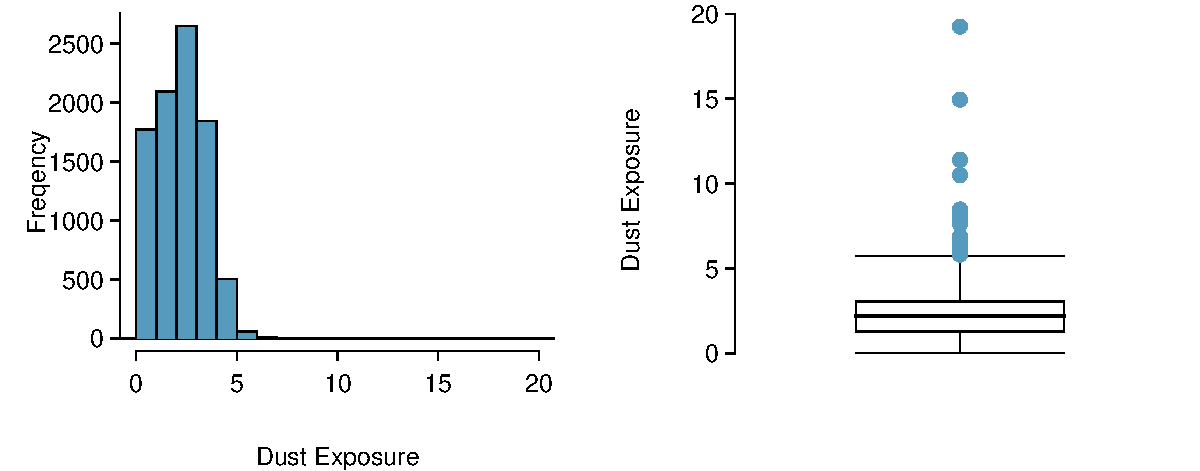
\includegraphics[width = \textwidth]{ch_inference_foundations_oi_biostat/figures/histOfDustExposure/histOfDustExposure}
\caption{Distribution of the dust exposure among 8936 coal miners. The box plot shows that these data are skewed. The distribution has an extremely long right tail. However, there are only approximately 70 outliers resulting in moderate skewness, exaggerating the skewness in the histogram.}
\index{skew!example: moderate}
\label{histOfDustExposure}
\end{figure}

Before moving onto Step 2 in the hypothesis testing framework, conditions for normality must be verified. (1)~There is no obvious evidence in the paper that the authors did not include randomness in sampling. Observations can be considered independent. (2) The sample size is sufficiently large as it is greater than 30. (3) The data show moderate skew in Figure ~\ref{histOfDustExposure} with the presence of a few outliers. This skew and the outliers (which are not too extreme) are acceptable for a sample size of $n=8936$ \footnote{Data is almost never collected perfectly. There generally exists error be it sampling error or measurement error within the data. Having a larger sample size mitigates large effects on inference.}. With these conditions verified, the normal model can be safely applied to $\overline{\mathrm{dust}}$ and the estimated standard error will be accurate.

\begin{exercise} \label{findSEOfFirstSleepStudyCheckingGreaterThan7Hours}
What is the standard deviation associated with $\overline{\mathrm{dust}}$? That is, estimate the standard error of $\overline{\mathrm{dust}}$.\footnote{The standard error can be estimated from the sample standard deviation and the sample size: $SE_{\overline{\mathrm{dust}}} = \frac{s_\mathrm{dust}}{\sqrt{n}} = \frac{1.23}{\sqrt{8936}} = 0.013$.}
\end{exercise}

The hypothesis test will be evaluated using the standard significance level $\alpha = 0.05$. The sampling distribution assumes that the null hypothesis is true. In this case, the sample mean, 2.20 hours, was drawn from a distribution that is nearly normal with mean 2 and standard deviation of about 0.013. Such a distribution is shown in Figure ~\ref{pValueOneSidedCoalStudy}. 

\begin{figure}[hht]
   \centering
   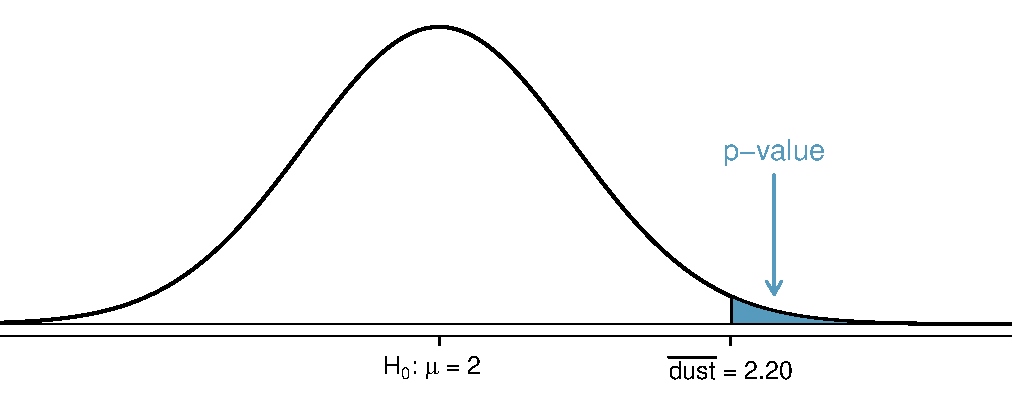
\includegraphics[width=0.73\textwidth]{ch_inference_foundations_oi_biostat/figures/pValueOneSidedCoalStudy/pValueOneSidedCoalStudy}
  \caption{Assuming the null hypothesis is true, the sample mean $\overline{\mathrm{dust}}$ is from this nearly normal distribution. The right tail describes the probability of observing such a large sample mean if the null hypothesis is true. The p-value is the shaded blue area that is more extreme than $\overline{\mathrm{dust}}$. All means larger than the sample mean are more favorable to the alternative hypothesis than the observed mean.}
\label{pValueOneSidedCoalStudy}
\end{figure}

Step 3 is the calculation of the T-statistic for sample mean $\overline{\mathrm{dust}} = 2.20$. 
\[ T = \frac{\overline{\mathrm{dust}} - \text{null value}}{SE_{\overline{\mathrm{dust}}}} = \frac{2.20 -2}{0.013} = 15.35\]

The T-statistic is calculated to equal 15.35 and can be approximated to the normal distribution with $n=8936$. The normal table on Page ~\pageref{normalProbabilityTable} does not list a Z-scores larger than 3.4 in absolute value. The NIOSH turns to \textsf{R}, 
 \begin{verbatim} 
 > 1-pnorm(15.35)
[1] 0 
\end{verbatim}
The area to the right of 15.35 in a normal distribution cannot equal exactly 0 from the section on the normal distribution in Chapter ~\ref{modeling}. However the area is so microscopic that \textsf{R} approximates it to 0. 

{\em If the null hypothesis is true, the probability of observing such a large sample mean of 2.20 for a sample of 8936 students is almost 0.}
\index{p-value!interpretation example} That is, if the null hypothesis is true, such a large mean would not be observed in most\footnote{almost all} instances. 

Step 5 compares the p-value to the significance level. Because the p-value is less than the significance level $\alpha$, the null hypothesis is rejected.\footnote{Using critical values instead, for $\alpha=0.05$ and a one sided alternative, the critical value is 1.65. Since the T-statistic is greater than 1.65, $H_0$ is rejected without needing to calculate the p-value.} NIOSH's observation was so unusual with respect to the null hypothesis that it casts serious doubt on $H_0$ and provides strong evidence favoring $H_A$. In context, it is most likely that these mines did not meet federal regulations for dust exposure limits in 1992. 

\begin{tipBox}{\tipBoxTitle{It is useful to first draw a picture to find the p-value}
It is useful to draw a picture of the distribution of $\overline{x}$ as though $H_0$ was true (i.e. $\mu$ equals the null value), and shade the region (or regions) of sample means that are at least as favorable to the alternative hypothesis. The sum of the shaded regions represent the p-value.}
\end{tipBox}

\subsection{Testing hypotheses using confidence intervals}
\label{utilizingOurCI}

Confidence intervals and hypothesis testing may seem disjointed -- one provides a range of values while the other results in a yes or no conclusion, but these two methods are arrive at the same conclusions to about a null hypothesis. 
	
\begin{example}{
The 2000 Census listed the median age of US adults as 35.3 years. With a simple random sample of 100 people from the \data{BRFSS} dataset, the CDC wants to see how its estimated population parameter compares with the one listed by the Census.  \footnote{The 2000 Census \url{https://www.census.gov/prod/2001pubs/c2kbr01-12.pdf} listed the median age instead of mean age. While the Census does not mention normality for the age distribution, the difference in mean and median age is negligible because the US population is so large.} The sample has an average age of 43.9 years and a sample standard deviation of 17.97 years. Conduct a hypothesis test and a confidence interval. Are these related in anyway?}
\label{CIandHypTests}

Beginning with hypothesis testing, the CDC first verifies the assumptions are met. With a sample size of $n=100$, independence and normality hold.  The null and alternative hypotheses are defined as: 
\begin{itemize}
\setlength{\itemsep}{0mm}
\item[$H_0$:] $\mu_{\mathrm{age}}=35.3$
\item[$H_A$:] $\mu_{\mathrm{age}} \neq 35.3$
\end{itemize}
The alternative hypothesis is two-sided because the CDC has no prior belief on the sidedness of this question. 

Let $\alpha$ = 0.05. The T-statistic is
 \[T = \frac{43.9-35.3}{17.97/\sqrt{100}}= \frac{8.6}{1.797} = 4.79\] With $n\geq 30$, the T-statistic can follow a normal distribution to calculate the p-value in \textsf{R}. The p-value is 
\begin{verbatim}
> 2*(1-pnorm(4.79))
[1] 1.667813e-06
\end{verbatim}

For a two-sided alternative, the p-value is less than $\alpha$. Therefore the sample that the CDC observed can be considered a "rare event" if the null hypothesis were true. Because the p-value is less than 0.05, the null hypothesis is rejected. Observing a sample mean of 43.9 years gives the CDC sufficient evidence that the average US adult age is not consistent with the Census estimate of 35.3 years old. 

The CDC then calculates a confidence interval. Under hypothesis testing, the CDC used $\alpha=0.05$, so the CDC chooses to create a 95\% confidence interval with the same sample. 

\begin{align*}
43.9 &\pm 1.96 * \frac{17.97}{\sqrt{100}}\\
43.9 &\pm 1.96 * 1.797\\
(40.38,& 47.42)\
\end{align*} 

The CDC is 95\% confident that the average age of all the US adults lies between 40.38 and 47.42 years after observing a sample mean of 43.9 years. The CDC notes that 35.3 years is not included in this interval, so there is sufficient evidence that the average age of the US adult population is not 35.3 years. 
\end{example}

The connection between confidence intervals and hypothesis testing is this: rejecting a null hypothesis for a two-sided alternative hypothesis corresponds to the null value not falling within the confidence interval. The equivalence only is true if the alternative hypothesis is two-sided and the significance levels for both are equal.

It is also important to note what this conclusion implies. Under this conclusion, the CDC should reject the Census's estimate of the average age. Intuitively, however, Census estimates seem more trustworthy simply because the estimate is from the Census. Even though statistical procedure is accurately followed, conclusions vary and could even be wrong. Understanding the context of the hypothesis testing and the data source becomes extremely important in practice.

\begin{exercise} \label{htForHousingExpenseForCommunityCollege650} \textbf{NEW EXMAPLE}
An investigator is studying the results of standardized IQ tests in adolescents who suffered from severe asthma during childhood. She claims that those who had childhood asthma perform worse than the population average. For the standardized test she will use, the mean score is 100. What are the null and alternative hypotheses to test whether this claim is accurate? \footnote{$H_0$: The average score is 100, $\mu = 100$. \hspace{3.4mm} $H_A$: The average score is lower than 100, $\mu \leq 100$.}
\end{exercise}

\begin{example}{In her sample of 100 children, she found a sample mean $\overline{x} = 96.7$ and standard deviation $s = 10$. Construct a 95\% confidence interval for the population mean and evaluate the hypotheses of Exercise~\ref{htForHousingExpenseForCommunityCollege650}.}
$$ SE = \frac{s}{\sqrt{n}} = \frac{10}{\sqrt{100}} = 1 $$
The normal model may be applied to the sample mean because the conditions are met: The data are a simple random sample and we assume that there are more than 1,000 adolescents who have suffered from asthma. The observations are independent and the sample size is also sufficiently large (n=100). The sample size mitigates potential effects of outliers even though the distribution is not provided. This ensures a 95\% confidence interval may be accurately constructed:
$$\overline{x}\ \pm\ z^{\star} SE \quad\to\quad 96.7\ \pm\ 1.96 \times  1 \quad \to \quad (94.74, 98.66) $$
Because the null value 100 does not lie within the confidence interval, a population mean score of 100 from all adolescents who suffered from sever asthma during childhood is implausible, and the null hypothesis is rejected. The data provide statistically significant evidence that adolescents who suffered from severe asthma during childhood do perform worse on standardized IQ tests. 
\end{example}

\textbf{NEWWWWW EXAMPLEEEEEEE}

\subsection{Decision errors}\label{DecisionErrors}

\index{hypothesis testing!decision errors|(}

Hypothesis tests are not flawless. Just think of the court system: innocent people are sometimes wrongly convicted. The guilty sometimes walk free. 

Similarly, scientists can make the wrong conclusions, induced by sampling variation, within hypothesis testing. However, the difference is that, unlike the court system, there exists tools necessary to quantify how often such errors are made. There are four possible scenarios in hypothesis test conclusions, which are summarized in Table~\ref{fourHTScenarios}.

\begin{table}[ht]
\centering
\begin{tabular}{l l c c}
& & \multicolumn{2}{c}{\textbf{Test conclusion}} \\
  \cline{3-4}
\vspace{-3.7mm} \\
& & do not reject $H_0$ &  reject $H_0$ in favor of $H_A$ \\
  \cline{2-4}
\vspace{-3.7mm} \\
& $H_0$ true & correct &  Type~1 Error \\
\raisebox{1.5ex}{\textbf{Truth}} & $H_A$ true & Type 2 Error & correct \\
  \cline{2-4}
\end{tabular}
\caption{Four different scenarios for hypothesis tests.}
\label{fourHTScenarios}
\end{table}

A \term{Type~1 Error} is rejecting the null hypothesis when $H_0$ is actually true. A \term{Type~2 Error} is failing to reject the null hypothesis when the alternative is actually true.

\begin{exercise} \label{whatAreTheErrorTypesInUSCourts}
In a US court, the defendant is either innocent ($H_0$) or  guilty ($H_A$). What does a Type~1 Error represent in this context? What does a Type 2 Error represent? Table~\ref{fourHTScenarios} may be useful. Disregard mistrials and hung juries. \footnote{If the court makes a Type~1 Error, this means the defendant is innocent ($H_0$ true) but wrongly convicted. A Type 2 Error means the court failed to reject $H_0$ (i.e. failed to convict the person) when the defendant was, in fact, guilty ($H_A$ true).}
\end{exercise}

\begin{exercise} \label{howToReduceType1ErrorsInUSCourts}
How could US courts reduce the Type~1 Error rate? What influence would this have on the Type 2 Error rate?\footnote{To lower the Type~1 Error rate (incorrect convictions), the standard conviction could be raised from ``beyond a reasonable doubt'' to ``beyond a conceivable doubt'' so fewer people would be wrongly convicted. However, there exists a tradeoff. By increasing the threshold, it would make it more difficult to convince people who are guilty. By reducing the Type~1 Error rate, the US courts would increase the Type 2 Error rate.}
\end{exercise}

\begin{exercise} \label{howToReduceType2ErrorsInUSCourts}
How could Type~2 Error rate be reduced in US courts? What influence would this have on the Type~1 Error rate?\footnote{A Type~2 Error occurs when the US court does not convict a guilty defendant. A decrease in Type~2 Error results in the US courts correctly convicting more guilty individuals. The standard of conviction could be lowered from ``beyond a reasonable doubt'' to ``beyond a little doubt'' to achieve this. Lowering the bar for guilt, however, results in more wrongful convictions, raising the Type~1 Error rate.}
\end{exercise}

\begin{exercise} \label{errorsinHIVTesting}
Consider a person getting tested for HIV. What do a Type~1 and Type~2 Error represent in this context? \footnote{Type~1 Error is if this person does not have HIV but was tested positive for HIV. Type~2 Error would be failing to detect HIV when the patient actually has HIV. }
\end{exercise}

\index{hypothesis testing!decision errors|)}

Exercises~\ref{whatAreTheErrorTypesInUSCourts} and ~\ref{howToReduceType2ErrorsInUSCourts} provide an important lesson: if one type of error is reduced, the other error type is generally increased. 

Hypothesis testing is built around rejecting or failing to reject the null hypothesis from strong evidence. But what does \emph{strong evidence} mean? In hypothesis testing, a p-value less than $\alpha$ provides strong evidence to reject the null hypothesis. Section ~\ref{hypothesisFramework} first introduced the relationship between $\alpha$ and Type 1 Error. This value for $\alpha$, the \term{significance level}, \index{hypothesis testing!significance level}  \marginpar[\raggedright\vspace{-4mm} $\alpha$\\\footnotesize significance\\level of a\\hypothesis test]{\raggedright\vspace{-4mm} $\alpha$\\\footnotesize significance\\level of a\\hypothesis test} is interpreted as the probability that scientists commit a Type 1 Error. That is, for $\alpha=0.05$, when $H_0$ is true, scientists do not want to incorrectly reject $H_0$ more than 5\% of the time. 

Hypothesis testing can occur in all industries ranging from manufacturing to medical testing. The question remains: which error type do they want to reduce the most? In general, the hypotheses and testing implications will determine if reducing Type 1 Error is more or less desirable than reducing Type 2 Error. The testing context will also determine which level of $\alpha$ scientists want to choose. Different significance levels beyond $\alpha = 0.05$ will be discussed in Section~\ref{significanceLevel}. However the significance level chosen depends on the study's threshold for committing a Type 1 Error and allowing a Type 2 Error. 

\subsection{Two-sided versus one-sided hypothesis testing: dos and don'ts}
\label{twoSidedTestsWithPValues}

\index{data!school sleep|(}

Students and scientists alike have the urge to reject the null hypothesis. In many instances, the null hypothesis is stated as the status quo. Rejecting the null hypothesis allows scientists, after spending time and resources, to make an important contribution to the field with a new discovery. 

The conclusion of a hypothesis test depends largely on the p-value and the alternative hypothesis. Determining an alternative hypothesis can get tricky, and the choice between a one-sided and two sided test can be controversial. Most importantly, it is never okay to change two-sided tests to one-sided tests after observing the data. The following exercise considers the consequences of switching mid-process.

\begin{exercise} 
Like Example ~\ref{onesidedCoalExample}, a second group of researchers randomly sampled 200 miners across the US in 1992. They were interested in whether their sample of miners differed from the dust exposure limit of 2 $\mathrm{mg}/\mathrm{m}^3$. Write the null and alternative hypotheses for this investigation.\footnote{Because the researchers are interested in any difference, they should use a two-sided alternative: $H_0: \mu = 2$, $H_A: \mu \neq 2$.}
\label{2ndCoalHypSetupExercise}
\end{exercise}

\begin{example}{The second group of researchers random samples 200 students and finds a mine of $\overline{x}=2.14 \mathrm{mg}/\mathrm{m}^3$ and a standard deviation of $s=1.15 \mathrm{mg}/\mathrm{m}^3$. Does this provide strong evidence against $H_0$ in Exercise~\ref{2ndCoalHypSetupExercise}? Use a significance level of $\alpha=0.05$.}
First, assumptions must be verified. (1) A simple random sample of less than 10\% of all miners in the US means the observations are independent. (2) The sample size is 200, which is greater than 30. (3) Although the distribution about dust exposures is unknown, a sample size of 200 surely allows the sample mean to be normally distributed with outliers and skewness having little effect. 

Next compute the standard error ($SE_{\overline{x}} = \frac{s}{\sqrt{n}} = 0.08$) of the estimate and create a picture to represent the p-value, shown in Figure~\ref{2ndSchSleepHTExample}. Both tails are shaded since the alternative hypothesis provided in Exercise \ref{2ndCoalHypSetupExercise} is two-sided.

Calculate the tail areas by first finding the lower tail corresponding to $\overline{x}$:
\begin{eqnarray*}
T = \frac{2.14 - 2}{0.08} = 1.75 \quad\stackrel{\text{table or \textsf{R}}}{\rightarrow}\quad \text{left tail}=0.04
\end{eqnarray*}
Because the normal model is symmetric, the right tail will have the same area as the left tail. The p-value is found as the sum of the two shaded tails:
\begin{eqnarray*}
\text{p-value} = \text{left tail} + \text{right tail} = 2\times(\text{left tail}) = 0.08
\end{eqnarray*}
This p-value is is larger than $\alpha=0.05$, so $H_0$ should not be rejected. That is, if $H_0$ is true, it would not be very unusual to see a sample mean this far from 2 $\mathrm{mg}/\mathrm{m}^3$ simply due to sampling variation. There is not sufficient evidence to conclude that the mean is different from 2 $\mathrm{mg}/\mathrm{m}^3$ and the mines seem to be following the law.

However, consider if this second group of researchers switched to a one-sided alternative hypothesis before the T-statistic was calculated. Keeping the sample and all other values the same, the p-value under a one-sided alternative would be 0.04. This new p-value is less than $\alpha = 0.05$ and would result in $H_0$ being rejected, a different conclusion than with the two-sided alternative. 
\index{data!school sleep|)}
\end{example}

Exercise ~\ref{2ndCoalHypSetupExercise} introduces the dangers of switching alternative hypothesis after observing the data, especially when p-values are close to $\alpha$. In practice, research that concludes using a p-value close to $\alpha$ warrants some skepticism. A p-value of 0.048 is not so different from a p-value of 0.052 but results in very different conclusions. Instead, another study should be conducted. The next example shows that freely switching from two-sided tests to one-sided tests will cause researchers to make twice as many Type~1 Errors as intended.

\begin{example}{Consider two cases: (1) The sample mean is larger than the null value and (2) the sample mean is smaller than the null value. 

(1) Suppose the sample mean was larger than the null value, $\mu_0$ (e.g. $\mu_0$ would represent~2 if $H_0$:~$\mu = 2$). Then the researchers could flipped to a one-sided test instead of a two-sided test, they would use $H_A$: $\mu > \mu_0$ after observing the data\footnote{They opt to minimize the Type~1 Errors}. Any T-statistic greater than 1.65 would result in rejecting $H_0$. If the null hypothesis is true, the large T-statistic would result in incorrectly rejecting the null hypothesis about 5\% of the time when the sample mean is above the null value, as shown in Figure~\ref{type1ErrorDoublingExampleFigure}.

(2) Suppose the sample mean was smaller than the null value. The researchers would choose $H_A$: $\mu < \mu_0$ if they could change to a one-sided test. If $\overline{x}$ had a T-statistic smaller than -1.65, $H_0$ would be rejected. If the null hypothesis is true, $H_0$ would be incorrectly rejected about 5\% of the time.}

Putting these two scenarios together, if the researchers were free to switch alternative hypotheses after observing the data, the Type~1 Error rate would be $5\%+5\%=10\%$ of the time instead of the specified $\alpha = 0.05$. This is twice the error rate we prescribed with our significance level of 0.05! 

\begin{figure}
   \centering
   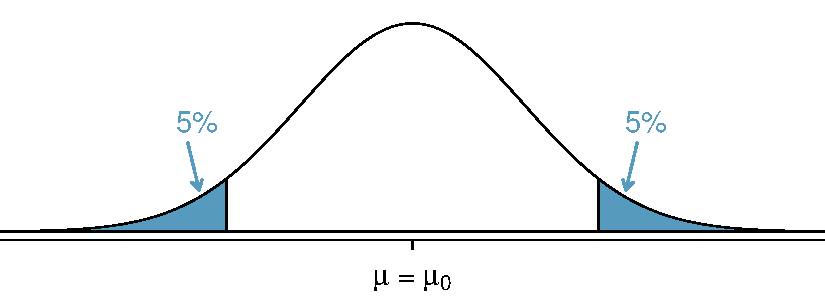
\includegraphics[width=0.7\textwidth]{ch_inference_foundations_oi_biostat/figures/type1ErrorDoublingExampleFigure/type1ErrorDoublingExampleFigure}
   \caption{The shaded regions represent areas where we would reject $H_0$ under the bad practices considered in Example~\ref{swappingHypAfterDataDoublesType1ErrorRate} when $\alpha = 0.05$.}
   \label{type1ErrorDoublingExampleFigure}
\end{figure}

\end{example}

This examples and exercises in this text will be obvious enough to decide on an alternative hypothesis. In practice, however, it can be less straightforward. If the sidedness is uncertain, many scientists opt to use a two-sided alternative because it is more \emph{conservative}. What does conservative in this context mean? Exercise ~\ref{2ndCoalHypSetupExercise} and the previous example showed that the two-sided tests would fail to reject the null hypothesis more often. The p-value for a two-sided alternative is twice as large producing a "safer" and more conservative hypothesis test conclusion. 

\begin{caution}{One-sided hypotheses are allowed only \emph{before} seeing data}
{After observing data, it is tempting to turn a two-sided test into a one-sided test resulting in a statistically significant one-sided conclusion. Avoid this temptation. Remember, the direction of a one-sided test must be made a priori, \emph{before} observing the data. If~they are not, the test must be two-sided.}
\end{caution}

\subsection{Choosing a significance level}
\label{significanceLevel}

\index{hypothesis testing!significance level|(}
\index{significance level|(}

Choosing a significance level for a hypothesis test is important. Traditionally, the $\alpha$ level is $0.05$. However, it is often helpful to adjust the significance level based on the application and on the consequences of the test's potential conclusions.

If making a Type~1 Error is dangerous or especially costly, a small significance level (e.g. smaller than 0.05) should be chosen. The study should demand very strong evidence favoring $H_A$ before $H_0$ is rejected. Many would use $\alpha=0.01$ or some value similar in this situation. 

If a Type 2 Error is relatively more dangerous or more costly than a Type~1 Error, a higher significance level (e.g. 0.10) should be chosen. Hypothesis tests should be cautious about failing to reject $H_0$ when the null is actually false.  Section~\ref{sampleSizeAndPower} will discuss this case in more detail.

\begin{tipBox}{\tipBoxTitle[]{Significance levels should reflect consequences of errors}
The significance level selected for a test should reflect the consequences associated with Type~1 and Type 2 Errors.}
\end{tipBox}

\begin{example}{A medical machine manufacturer is considering a higher quality but more expensive supplier for parts in making an MRI. The engineers sample a number of parts from the current supplier and also parts from the new supplier. They decide that if the high quality parts will last more than 10\% longer, it makes financial sense to switch to this more expensive supplier. Is there good reason to modify the significance level in such a hypothesis test?}
The null hypothesis is that the more expensive parts last no more than 10\% longer while the alternative is that they do last more than 10\% longer. This decision is just one of the many regular factors that impact the MRI and the company's financial health. A significance level of 0.05 seems reasonable since neither a Type~1 or Type 2 error should be dangerous or (relatively) much more expensive. The machine's accuracy will not be affected by a change in supplier.
\end{example}

\begin{example}{Now the same MRI manufacturer is considering a slightly more expensive supplier for parts related to accuracy not longevity. If the accuracy of the machine's components is shown to be better than the current supplier, they will switch manufacturers. Is there good reason to modify the significance level from $\alpha=0.05$ in such an evaluation?}
The null hypothesis would be that the suppliers' parts are equally reliable and equally accurate in detection. Because safety is involved, the MRI machine company should be eager to switch to the slightly more expensive manufacturer (reject $H_0$) even if the evidence of increased safety and effectiveness is only moderately strong. A slightly larger significance level, such as $\alpha=0.10$, might be appropriate.
\end{example}

\begin{exercise}
A specific part inside of an MRI machine is very expensive to replace. However, the machine usually functions properly even if this part is broken; the machine detects the most common injuries at the same probability with a broken part. The part is replaced only if the doctors are extremely certain it is broken based on a series of measurements. Identify appropriate hypotheses for this test (in plain language) and suggest an appropriate significance level.\footnote{The null hypothesis is that the part is not broken, and the alternative is that it is broken. If there is not sufficient evidence to reject $H_0$, the part will not be replaced. Failing to fix the part if it is broken ($H_0$ false, $H_A$ true) is not very problematic for common injuries, and replacing the part is expensive. Thus, very strong evidence against $H_0$ should exist before we replace the part. Choose a small significance level, such as $\alpha=0.01$.}
\end{exercise}

\index{significance level|)}
\index{hypothesis testing!significance level|)}
\index{hypothesis testing|)}

%__________________

\section{A Primer on the $t$-distribution}
\label{tdistribution}

Section ~\ref{hypothesisTesting} introduced the T-statistic as distributed according to the $t$-distribution. Section ~\ref{pValue} offered a rule of thumb that for $n\geq30$, the p-value of a $t$-distribution becomes almost indistinguishable from the p-value of a normal distribution. However, the characteristics of a $t$-distribution have yet to be explained. The properties of the $t$-distribution are not needed to perform hypothesis testing. However this section introduces the $t$-distribution and its characteristics at a more theoretical level.

\subsection{Introducing the $t$-distribution}
\label{introducingTheTDistribution}

\index{t-distribution|(}
\index{distribution!$t$|(}

In the cases where a small sample ($n<30$) is used to calculate the T-statistic, the $t$-distribution is a useful distribution for inference calculations. A $t$-distribution, shown as a solid line in Figure~\ref{tDistCompareToNormalDist}, has a bell shape. However, its tails are thicker than the tails in a normal model. This means observations are more likely to fall beyond two standard deviations from the mean than under the normal distribution.\footnote{It is useful to think of the $t$-distribution as having a standard deviation of 1 even though the standard deviation of the $t$-distribution is slightly more than 1.} These extra thick tails of the $t$-distribution are exactly the correction needed to resolve the problem of a poorly estimated standard error from a small sample.

\begin{figure}
\centering
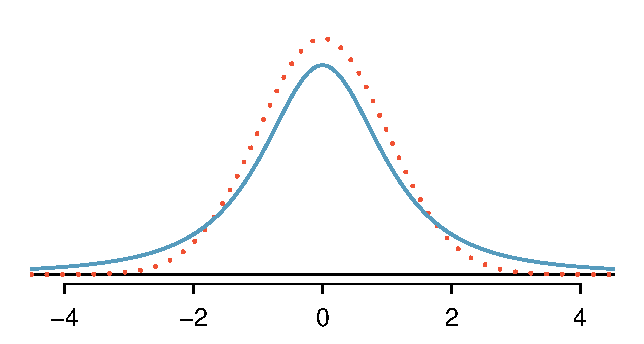
\includegraphics[width = \textwidth]{ch_inference_foundations_oi_biostat/figures/tDistCompareToNormalDist/tDistCompareToNormalDist}
\caption{Comparison of a $t$-distribution (solid line) to a normal distribution (dotted line).}
\label{tDistCompareToNormalDist}
\end{figure}

The $t$-distribution, always centered at zero, has a single parameter: degrees of freedom. The \termsub{degrees of freedom (df)}{degrees of freedom (df)!$t$-distribution} describe the precise form of the bell-shaped $t$-distribution. Several $t$-distributions are shown in Figure~\ref{tDistConvergeToNormalDist}. With more degrees of freedom, the $t$-distribution looks very much like the standard normal distribution. The degrees of freedom is $n-1$ where $n$ is the sample size for T-statistics from one sample. 

\begin{figure}
\centering
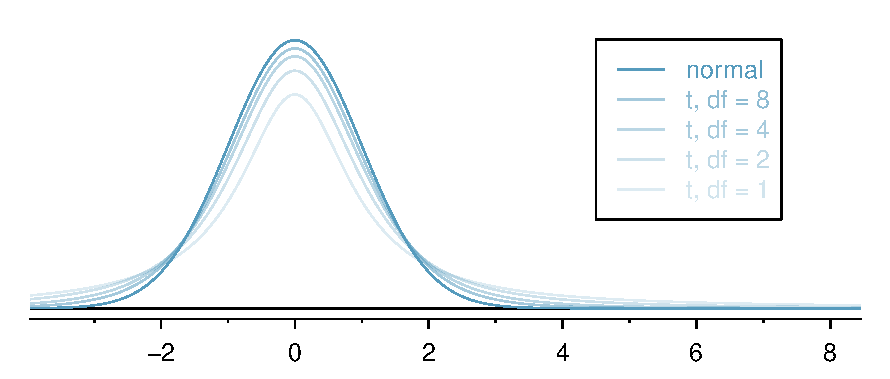
\includegraphics[width=\textwidth]{ch_inference_foundations_oi_biostat/figures/tDistConvergeToNormalDist/tDistConvergeToNormalDist}
\caption{The larger the degrees of freedom, the more closely the $t$-distribution resembles the standard normal model.}
\label{tDistConvergeToNormalDist}
\end{figure}

\begin{termBox}{\tBoxTitle{Degrees of freedom (df)}
The degrees of freedom describe the shape of the $t$-distribution. The larger the degrees of freedom, the more closely the distribution approximates the normal model.}
\end{termBox}

When the degrees of freedom is about 30 or more, the $t$-distribution is nearly indistinguishable from the normal distribution. 

It's very useful to become familiar with the $t$-distribution, because it allows greater flexibility than the normal distribution when analyzing numerical data. The \term{t-table}, partially shown in Table~\ref{tTableSample}, is used in place of the normal probability table. A larger $t$-table is in Appendix~\ref{tDistributionTable} on page~\pageref{tDistributionTable}. In~practice, it's more common to use statistical software like \textsf{R} instead of a table. 
\begin{table}[hht]
\centering
\begin{tabular}{r | rrr rr}
one tail & \hspace{1.5mm}  0.100 & \hspace{1.5mm} 0.050 & \hspace{1.5mm} 0.025 & \hspace{1.5mm} 0.010 & \hspace{1.5mm} 0.005  \\
two tails & 0.200 & 0.100 & 0.050 & 0.020 & 0.010 \\
\hline
{$df$} \hfill 1  &  {\normalsize  3.08} & {\normalsize  6.31} & {\normalsize 12.71} & {\normalsize 31.82} & {\normalsize 63.66}  \\ 
2  &  {\normalsize  1.89} & {\normalsize  2.92} & {\normalsize  4.30} & {\normalsize  6.96} & {\normalsize  9.92}  \\ 
3  &  {\normalsize  1.64} & {\normalsize  2.35} & {\normalsize  3.18} & {\normalsize  4.54} & {\normalsize  5.84}  \\ 
$\vdots$ & $\vdots$ &$\vdots$ &$\vdots$ &$\vdots$ & \\
17  &  {\normalsize  1.33} & {\normalsize  1.74} & {\normalsize  2.11} & {\normalsize  2.57} & {\normalsize  2.90}  \\ 
\highlightO{18}  &  \highlightO{\normalsize  1.33} & \highlightO{\normalsize  1.73} & \highlightO{\normalsize  2.10} & \highlightO{\normalsize  2.55} & \highlightO{\normalsize  2.88}  \\ 
19  &  {\normalsize  1.33} & {\normalsize  1.73} & {\normalsize  2.09} & {\normalsize  2.54} & {\normalsize  2.86}  \\ 
20  &  {\normalsize  1.33} & {\normalsize  1.72} & {\normalsize  2.09} & {\normalsize  2.53} & {\normalsize  2.85}  \\ 
$\vdots$ & $\vdots$ &$\vdots$ &$\vdots$ &$\vdots$ & \\
400  &  {\normalsize  1.28} & {\normalsize  1.65} & {\normalsize  1.97} & {\normalsize  2.34} & {\normalsize  2.59}  \\ 
500  &  {\normalsize  1.28} & {\normalsize  1.65} & {\normalsize  1.96} & {\normalsize  2.33} & {\normalsize  2.59}  \\ 
$\infty$  &  {\normalsize  1.28} & {\normalsize  1.64} & {\normalsize  1.96} & {\normalsize  2.33} & {\normalsize  2.58}  \\ 
\end{tabular}
\caption{An abbreviated look at the $t$-table. Each row represents a different $t$-distribution. The columns describe the cutoffs for specific tail areas. The row with $df=18$ has been \highlightO{highlighted}.}
\label{tTableSample}
\end{table}

Each row in the $t$-table represents a $t$-distribution with different degrees of freedom. The columns correspond to tail probabilities. For instance, if $df=18$, researchers can examine row 18, which is highlighted in Table~\ref{tTableSample}. If researchers instead want the value in this row that identifies the cutoff for an upper tail of 10\%, they can look in the column where \emph{one tail} is 0.100. This cutoff is 1.33. If they had wanted the cutoff for the lower 10\%, they would use -1.33. Just like the normal distribution, $t$-distributions are symmetric.

\begin{example}{What proportion of the $t$-distribution with 18 degrees of freedom falls below -2.10?}
Just like a normal probability problem, Figure~\ref{tDistDF18LeftTail2Point10} provides a picture with the shaded area below -2.10. To find this area, the appropriate row needs to be identified in the $t$-table: \mbox{$df=18$}. 
Then identify the column containing the absolute value of -2.10; it~is the third column. The shaded area is only one tale, and the top line of the table shows that a one tail area for a value in the third row corresponds to 0.025. About 2.5\% of the distribution falls below -2.10. The next example encounters a case where the exact $t$ value is not listed in the table where \textsf{R} would provide more use.
\end{example}

\begin{figure}
\centering
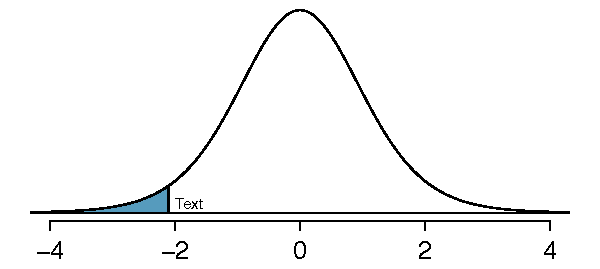
\includegraphics[width=0.5\textwidth]{ch_inference_foundations_oi_biostat/figures/tDistDF18LeftTail2Point10/tDistDF18LeftTail2Point10}
\caption{The $t$-distribution with 18 degrees of freedom. The area below -2.10 has been shaded.}
\label{tDistDF18LeftTail2Point10}
\end{figure}

\begin{example}{A $t$-distribution with 20 degrees of freedom is shown in the left panel of Figure~\ref{tDistDF20RightTail1Point65}. Estimate the proportion of the distribution falling above 1.65.}
Looking at the $t$-table again, identify the row using the degrees of freedom: $df=20$. Then look for 1.65; it is not listed. It falls between the first and second columns. Since these values bound 1.65, their tail areas will bound the tail area corresponding to 1.65. One tail area of the first and second columns -- 0.050 and 0.10 --concluded that between 5\% and 10\% of the distribution is more than 1.65 standard deviations above the mean. However this is only an estimation. Statistical software like \textsf{R} can provide more precision \begin{verbatim}
> 1-pt(1.65,20)
[1] 0.05728041
\end{verbatim}
where \var{pt()} calculates the shaded area left of 1.65 of a $t$-distribution with 20 degrees of freedom. The shaded area is 0.0573. 
\end{example}

\begin{figure}
\centering
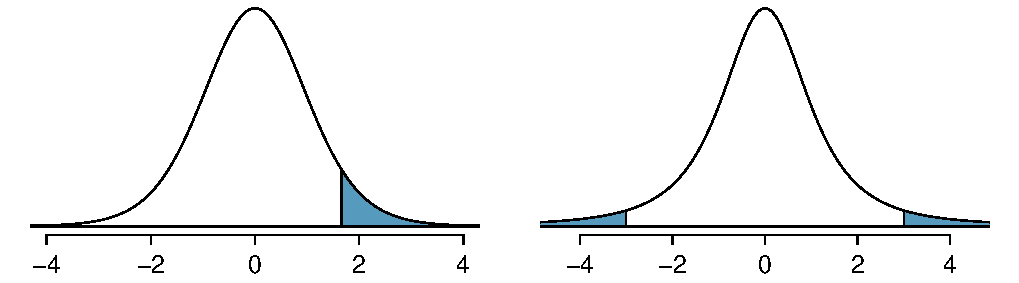
\includegraphics[width=0.85\textwidth]{ch_inference_foundations_oi_biostat/figures/tDistDF20RightTail1Point65/tDistDF20RightTail1Point65}
\caption{Left: The $t$-distribution with 20 degrees of freedom, with the area above 1.65 shaded. Right: The $t$-distribution with 2 degrees of freedom, with the area further than 3 units from 0 shaded.}
\label{tDistDF20RightTail1Point65}
\end{figure}

\begin{example}{A $t$-distribution with 2 degrees of freedom is shown in the right panel of Figure~\ref{tDistDF20RightTail1Point65}. Estimate the proportion of the distribution falling more than 3 units from the mean (above or below).}
As before, first identify the appropriate row: $df=2$. Next, find the columns that capture 3; because $2.92 < 3 < 4.30$, use the second and third columns. Finally, 0.05 and 0.1 are the bounds for the tail areas under "two tails" since the $t$-distribution is symmetric. For more precision, \textsf{R} outputs 
\begin{verbatim} > 2*pt(-3, 2)
[1] 0.09546597
\end{verbatim}
\end{example}

\begin{exercise}
What proportion of the $t$-distribution with 19 degrees of freedom falls above -1.79 units?\footnote{Shade area \emph{above} -1.79 on a symmetric distribution (the picture is left to you). The small left tail is between 0.025 and 0.05, so the larger upper region must have an area between 0.95 and 0.975 (1 - the small left tail area). Using \textsf{R} again, > 1-pt(-1.79, 19) [1] 0.9552978}

\index{distribution!$t$|)}
\index{t-distribution|)}

\end{exercise}

\subsection{Conditions for using the $t$-distribution for inference on a sample mean}
\label{tDistSolutionToSEProblem}

To infer on a single mean using the $t$-distribution, two conditions need to be checked. These assumptions are the same for a normal distribution as well.
\begin{description}
\item[Independence of observations.] This condition was verified before in Section ~\ref{changingTheConfidenceLevelSection} as a condition that $\overline{x}$ is nearly normal. The sample should be taken from less than 10\% of the population as a simple random sample. If the data are from an experiment or random process, the observations should be independent. 
\item[Observations come from a nearly normal distribution.] This second condition is difficult to verify with small data sets. To diagnose (i) take a look at a plot of the data for obvious departures from the normal model, and (ii) consider any previous experiences in which the data may not be nearly normal. \footnote{A large enough sample size can sometimes counteract concerns with skewness and make this assumption more lenient.}
\end{description}
When examining a sample mean and estimated standard error from a sample of $n$ independent and nearly normal observations, a $t$-distribution with $n-1$ degrees of freedom~($df$) can be used. For example, if the sample size was 19, then the $t$-distribution would have $df=19-1=18$ degrees of freedom and proceed exactly as in the rest of Chapter~\ref{foundationsForInference}, except now \emph{ the $t$-distribution is used}.

\begin{tipBox}{\tipBoxTitle{When to use the $t$-distribution}
Use the $t$-distribution to infer on the sample mean when observations are independent and nearly normal. The nearly normal condition is relaxed as the sample size increases. For example, the data distribution may be moderately skewed when the sample size is at least~30.}
\end{tipBox}







%__________________

\section{Examining the Central Limit Theorem closer (Special Topic)}
\label{cltSection}

\index{Central Limit Theorem|(}

Looking back to ~\ref{why30}, the normal model for the sample mean tends to be very good when the sample consists of at least 30 independent observations and the population data are not strongly skewed. The Central Limit Theorem provides the theory that allows this assumption to be made.

\begin{termBox}{\tBoxTitle{Central Limit Theorem, informal definition}
The distribution of $\overline{x}$ is approximately normal. The approximation can be poor if the sample size is small. However as $n$ increases, the sample mean becomes more and more normally distributed.}
\end{termBox}

Three theoretical cases will be considered to see roughly when the approximation is reasonable. Consider three data sets: one from a \emph{uniform} distribution, one from an \emph{exponential} distribution, and the other from a \emph{log-normal} distribution. Recall the properties of these distributions from Chapter ~\ref{modeling}. These distributions are shown in the top panels of Figure~\ref{cltSimulations}. The uniform distribution is symmetric, the exponential distribution may be considered moderately skewed since its right tail is relatively short (few outliers), and the log-normal distribution is strongly skewed and will tend to produce more apparent outliers.\index{skew!example: moderate}\index{skew!example: strong}

\begin{figure}
   \centering
   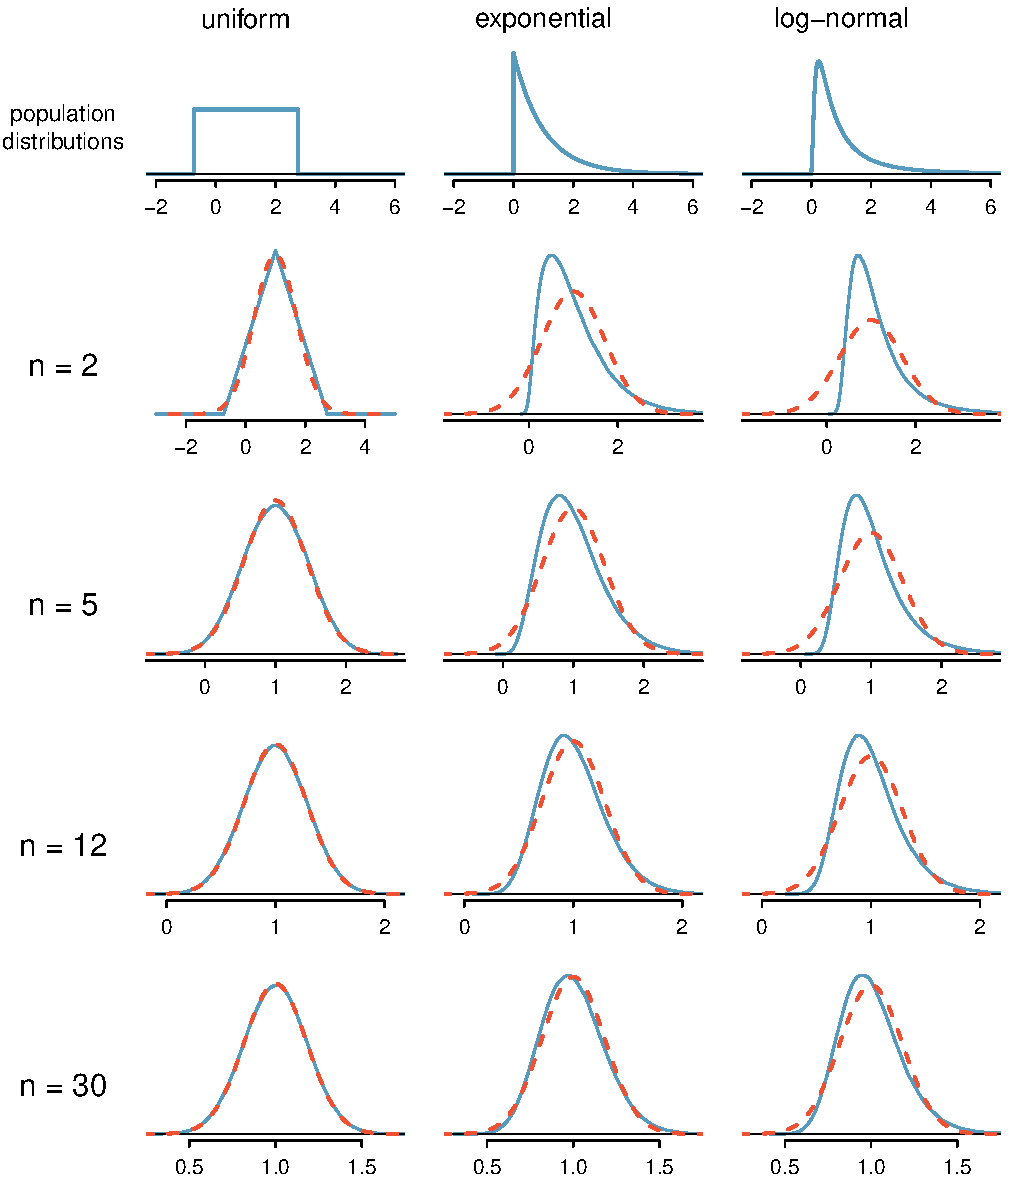
\includegraphics[width=\textwidth]{ch_inference_foundations_oi_biostat/figures/cltSimulations/cltSimulations}
   \caption{Sampling distributions for the mean at different sample sizes and for three different distributions. The dashed red lines show normal distributions.}
   \label{cltSimulations}
\end{figure}

The $n=2$ row represents the sampling distribution of $\overline{x}$ if $\overline{x}$ is the sample mean of two observations from each distribution. The dashed line represents the closest approximation of the normal distribution. 

\begin{exercise}
Examine the distributions in each row of Figure~\ref{cltSimulations}. As the sample size becomes larger, how does the normal approximation for each sampling distribution compare? \footnote{The normal approximation becomes better as larger samples are used.}
\end{exercise}

\begin{example}{Would the normal approximation be good in all applications where the sample size is at least 30?}
Not necessarily. The normal approximation for the log-normal example is questionable for a sample size of 30. The more skewed a population distribution or the more common the frequency of outliers, the larger the sample required to approximate the distribution of the sample mean to a normal distribution.
\end{example}

\begin{tipBox}{\tipBoxTitle{With larger $n$, the sampling distribution of $\overline{x}$ becomes more normal}
As the sample size increases, the normal model for $\overline{x}$ becomes more reasonable. The condition in skewness can be relaxed when the sample size is very large.}
\end{tipBox}


\begin{example}{Figure~\ref{pertussisTS} displays a histogram of 169 observations from a study published in \emph{Parasitology}\footnote{Magpantay FMG, Domenech de Cell�s M, Rohani P, King AA (2015) Pertussis immunity and epidemiology: mode and duration of vaccine-induced immunity. Parasitology, online in advance of print. \url{http://dx.doi.org/10.1017/S0031182015000979}} in 2015 on pertussis immunity \footnote{whooping cough}. This study investigated the nature and duration of vaccine protection to explain the resurgence of pertussis in countries with high vaccination coverage. The data, provided by the Italian Ministry of Health, is the number of monthly pertussis notification reports from 1996 to 2009 in selected regions in Italy. Figure ~\ref{pertussisTS} and figure ~\ref{pertussisHist} both use data from the Italian region Lombardia. Can the sample distribution of the sample mean, 23.07, be approximated to a normal or $t$ - distribution?}
Conditions first need to be verified. 
\begin{itemize}
\setlength{\itemsep}{0mm}
\item[(1)] These data are referred to as \term{time series data}, data that appears through time arriving in a particular sequence. 




If there were many Italians who contracted pertussis in one month, it would influence how many people would contract pertussis the next month. Pertussis is a highly contagious bacterial disease, so the number of monthly reports would presumably increase the month after many individuals contracted pertussis. Similarly if many Italians were vaccinated the month before, fewer people would be at risk of pertussis the following month. To make the assumption of independence, careful checks should be performed on such data. In many instances time series data are not independent. 
\item[(2)] The sample size is 169, satisfying the sample size condition.
\item[(3)] Figure ~\ref{pertussisHist} suggests that the data are very strongly skewed or very distant outliers may be common for this type of data. Outliers can play an important role and affect the distribution of the sample mean and the estimate of the standard error.
\end{itemize}
A normal distribution should not model the sample mean of these 169 observations because of the independence assumption. The very extreme skewness in Figure ~\ref{pertussisHist} also poses a challenge. \end{example}

\begin{figure}[ht]
   \centering
   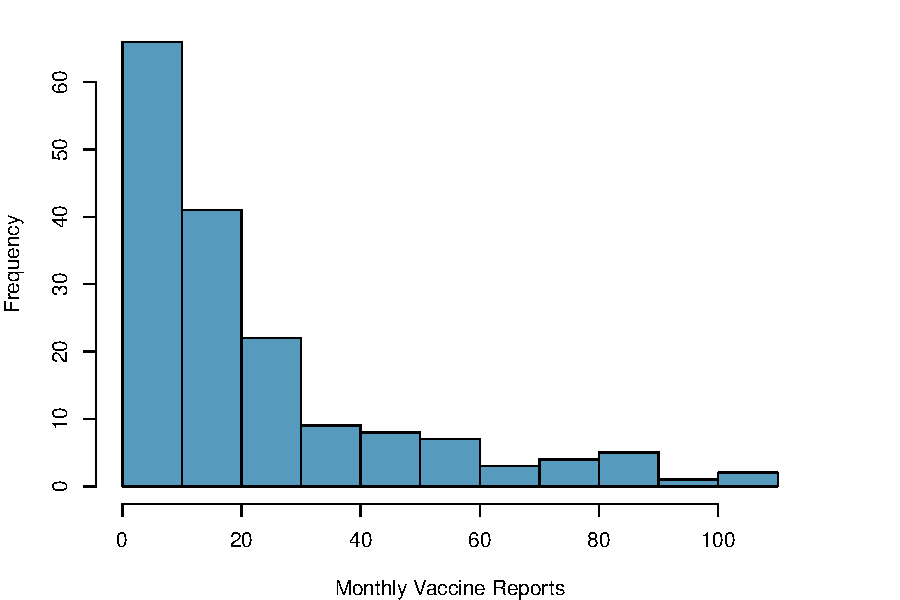
\includegraphics[width = \textwidth]{ch_inference_foundations_oi_biostat/figures/pertussisHist/pertussisHist}
   \caption{Histogram of the number of monthly reports every month from 1996 to 2009. These data include an obvious skewness. These are problematic when considering the normality of the sample mean. \index{skew!example: very strong}.}
   \label{pertussisHist}
\end{figure}

\begin{figure}[ht]
   \centering
   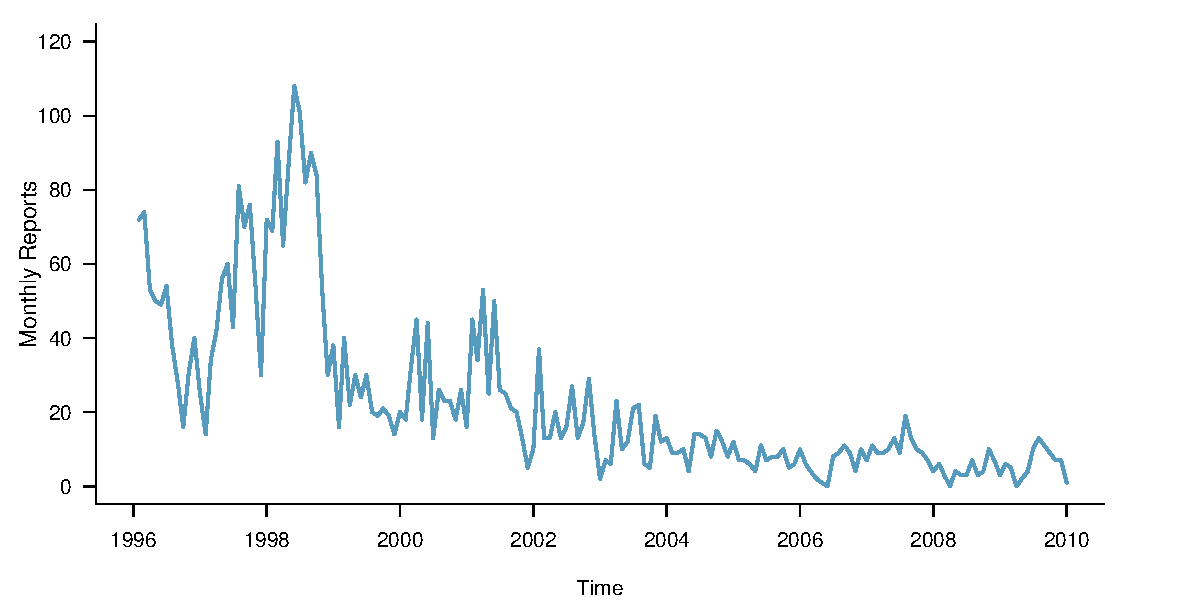
\includegraphics[width = \textwidth]{ch_inference_foundations_oi_biostat/figures/pertussisTS/pertussisTS}
   \caption{This is a plot depicting the time series, the number of monthly reports over time. Time series data is generally plotted like this because it is easy to see how values change over time.}
   \label{pertussisTS}
\end{figure}

\begin{caution}
{Examine data structure when considering independence}
{Some data sets are collected in such a way that they have a natural underlying structure between observations, e.g. when observations occur consecutively or they come from the same family etc. Be especially cautious about independence assumptions regarding such data sets.}
\end{caution}

\begin{caution}
{Watch out for strong skew and outliers}
{Strong skew is often identified by the presence of clear outliers. If a data set has prominent outliers, or such observations are somewhat common for the type of data under study, then it is useful to collect a sample with many more than 30 observations if the normal model will be used for $\overline{x}$. There are no simple guidelines for what sample size is big enough for all situations, so proceed with caution when working in the presence of strong skew or more extreme outliers.}
\index{skew!strongly skewed guideline}
\index{Central Limit Theorem|)}
\end{caution}











%__________________
\section{Inference for other estimators}
\label{aFrameworkForInference}

The sample mean is not the only point estimate for which the sampling distribution is nearly normal. The procedures introduced in Chapter ~\ref{foundationsForInference} are not limited to just estimating the population mean. The sampling distribution of sample proportions closely resembles the normal distribution when the sample size is sufficiently large. In this section, a number of examples will be introduced where the normal approximation is reasonable and procedures in this chapter can be applied to inference on other estimators. Chapters~\ref{inferenceForNumericalData} and~\ref{inferenceForCategoricalData} will revisit each of the point estimates in this section along with some other new statistics.

In order to use the tools introduced in Chapter ~\ref{foundationsForInference}, these point estimates need to obey some characteristics and assumptions. In addition to the assumptions encountered in this section, the estimate also needs to be unbiased. A point estimate is \term{unbiased} if the sampling distribution of the estimate is centered at the parameter it estimates. A biased point estimate consistently is too high or estimates are always always too low. That is, an unbiased estimate does not naturally over or underestimate the parameter. The sample mean is an example of an unbiased point estimate, as are each of the examples introduced in this section.

\subsection{Confidence intervals for nearly normal point estimates}

\index{confidence interval!using normal model|(}

In Section~\ref{confidenceIntervals}, the point estimate $\overline{x}$ with a standard error $SE_{\overline{x}}$ was used to create a 95\% confidence interval for the population mean:
\begin{align}
\overline{x}\ \pm\ 1.96 \times SE_{\overline{x}}
\label{95PercCIForMeanInGeneralizingSection}
\end{align}
This interval was constructed by noting that the sample mean is within 1.96 standard errors of the population mean 95\% of the time. This same logic generalizes to any unbiased point estimate that is nearly normal using a place-holder $z^{\star}$ for a confidence interval formula.

\begin{termBox}{\tBoxTitle{General confidence interval for the normal sampling distribution case}\label{generalConfidenceIntervalTermBox}%
For any unbiased point estimate, the confidence interval for a nearly normal point estimate is
\begin{eqnarray}
\text{point estimate}\ \pm\ z^{\star}SE
\label{95PercGeneralCIInGeneralizingSection}
\end{eqnarray}
$z^{\star}$ is selected to correspond to the confidence level, and $SE$ represents the standard error. $z^{\star}SE$ is called the \emph{margin of error}\index{margin of error}.}
\end{termBox}

In this section, the computed standard error for each example and exercise is provided without detailing where derivation. In future chapters, the formulae and other details for each scenario will elaborated upon.

\begin{example}{Using the \data{BRFSS BMI} data, the point estimate for the average difference in weights between men and women is $\overline{x}_\mathrm{{men}}-\overline{x}_\mathrm{{women}}= 36.61$ pounds. This point estimate is associated with a nearly normal distribution with SE = 0.35 pounds. What is a reasonable 95\% confidence interval for the difference in gender weights?}
\label{confIntervalForDifferenceOfRunTimeBetweenGenders}
The normal approximation is said to be valid, so apply Equation~\eqref{95PercGeneralCIInGeneralizingSection}:
\begin{eqnarray*}
\text{point estimate}\ \pm\ z^{\star} SE
	\quad\rightarrow\quad 36.61\ \pm\ 1.96\times 0.35
	\quad\rightarrow\quad (35.91, 37.31)
\end{eqnarray*}
Thus, scientists are 95\% confident that the men were, on average, between 35.91 to 37.31 pounds heavier than women. That is, the average difference among the population of men and women is plausibly between 35.91 and 37.31 pounds with 95\% confidence.
\end{example}

\begin{example}{Does Example~\ref{confIntervalForDifferenceOfRunTimeBetweenGenders} guarantee that if a husband and wife both weighed themselves, the husband would weigh between 35.91 and 37.31 pounds more than the wife?}
The confidence interval above says absolutely nothing about individual observations. It \emph{only} makes a statement about a plausible range of values for the \emph{average} difference between all men and all women in the US. 
\end{example}

\begin{exercise}
The proportion of men in the \data{BRFSS BMI} sample is $\hat{p}=0.42$. This sample meets certain conditions that ensure $\hat{p}$ will be nearly normal, and the standard error of the estimate is $SE_{\hat{p}}=0.05$. Create a 90\% confidence interval for the proportion of participants in the \data{BRFSS} study that will resemble the proportion of men in the US. \footnote{Use $z^{\star}=1.65$, and apply the general confidence interval formula:
\begin{eqnarray*}
\hat{p}\ \pm\ z^{\star}SE_{\hat{p}}
	\quad\to\quad 0.42\ \pm\ 1.65\times 0.05
	\quad\to\quad (0.3375, 0.5025)
\end{eqnarray*}
Thus, the CDC is 90\% confident that between 34\% and 50\% of the US adult population are men.}
\index{confidence interval!using normal model|)}
\end{exercise}

\subsection{Hypothesis testing for nearly normal point estimates}
\index{hypothesis testing!using normal model|(}

Hypothesis testing also applies to estimates that are unbiased and nearly normal. The following examples will only use the p-value approach introduced in Section ~\ref{pValue} and forgo the critical value shortcut.  

\begin{termBox}{\tBoxTitle[]{Hypothesis testing framework using the normal model}
\begin{enumerate}
\setlength{\itemsep}{0mm}
\item First write the hypotheses in plain language, then in mathematical notation using the appropriate point estimate and population parameter.
\item State a significance level $\alpha$. Generally use $\alpha=0.05$. 
\item Compute the test-statistic using the point estimate and standard error estimate. 
\item Calculate the p-value by drawing a picture of the sampling distribution under $H_0$. Know which area, according to the alternative, is being shaded to represent the correct p-value . 
\item Use the p-value to evaluate the hypotheses. Write a conclusion within the context of the problem. 
\end{enumerate}
} Conditions must be verified to ensure that the point estimate is nearly normal and unbiased so that the standard error estimate is also reasonable. This step can be done before computing the test-statistic.  
\end{termBox}

\begin{exercise} \label{fdaHypSetupForSulph}
A drug called sulphinpyrazone was under consideration for use in reducing the death rate in heart attack patients. To determine whether the drug was effective, a set of 1,475 patients were recruited into an experiment and randomly split into two groups: a control group that received a placebo and a treatment group that received the new drug. What would be an appropriate null hypothesis? And the alternative?\footnote{The skeptic's perspective is that the drug does not work at reducing deaths in heart attack patients ($H_0$), while the alternative is that the drug does work ($H_A$).}
\end{exercise}

Formalize the hypotheses from Exercise~\ref{fdaHypSetupForSulph} by letting $p_{control}$ and $p_{treatment}$ represent the proportion of patients who died in the control and treatment groups, respectively. Then the hypotheses can be written as
\begin{eqnarray*}
&&H_0: p_{control} = p_{treatment} \quad\text{(the drug does not work)} \quad \\
&&H_A: p_{control} > p_{treatment} \quad\text{(the drug works)}
\end{eqnarray*}
or equivalently,
\begin{eqnarray*}
&&H_0: p_{control} - p_{treatment} = 0 \quad\text{(the drug does not work)} \quad \\
&&H_A: p_{control} - p_{treatment} > 0 \quad\text{(the drug works)}
\end{eqnarray*}
Strong evidence against the null hypothesis and in favor of the alternative would correspond to an observed difference in death rates,
\begin{eqnarray*}
\text{point estimate} = \hat{p}_{control} - \hat{p}_{treatment}
\end{eqnarray*}
being larger than would be expected from chance alone. This difference in sample proportions represents a point estimate that is useful in evaluating the hypotheses. 

\begin{example}{Evaluate the hypothesis setup from Exericse~\ref{fdaHypSetupForSulph} using data from the study.\footnote{Anturane Reinfarction Trial Research Group. 1980. Sulfinpyrazone in the prevention of sudden death after myocardial infarction. New England Journal of Medicine 302(5):250-256.} In the control group, 60 of 742 patients died. In the treatment group, 41 of 733 patients died. The sample difference in death rates can be summarized as
\begin{eqnarray*}
\text{point estimate} = \hat{p}_{control} - \hat{p}_{treatment} = \frac{60}{742} - \frac{41}{733} = 0.025
\end{eqnarray*}
This point estimate is nearly normal and is an unbiased estimate. The standard error of this sample difference is $SE = 0.013$. Evaluate the hypothesis test at a 5\% significance level: $\alpha=0.05$.}
Identify the p-value to evaluate the hypotheses. If the null hypothesis is true, then the point estimate would have come from a nearly normal distribution, like the one shown in Figure~\ref{sulphStudyFindPValueUsingNormalApprox}. The distribution is centered at zero since $p_{control}-p_{treatment}=0$ under the null hypothesis. Because a large positive difference provides evidence against the null hypothesis and in favor of the alternative, the upper tail has been shaded to represent the p-value. The lower tail does not need to be shaded as this is a one-sided test: an observation in the lower tail does not support the alternative hypothesis.

\begin{figure}[bt]
   \centering
   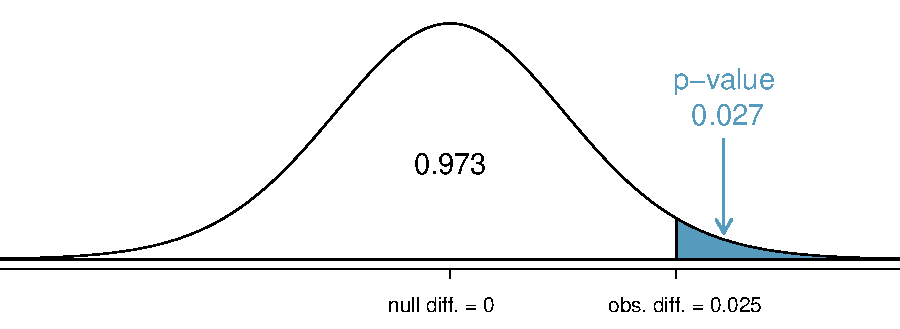
\includegraphics[height=37mm]{ch_inference_foundations_oi_biostat/figures/sulphStudyFindPValueUsingNormalApprox/sulphStudyFindPValueUsingNormalApprox}
   \caption{The distribution of the sample difference if the null hypothesis is true.}
   \label{sulphStudyFindPValueUsingNormalApprox}
\end{figure}

The p-value can be computed by using the Z score of the point estimate and the normal probability table.
\begin{eqnarray}
Z = \frac{\text{point estimate} - \text{null value}}{SE_{\text{point estimate}}}
	= \frac{0.025 - 0}{0.013} = 1.92
\label{zScoreOfPointEstimateForSulphinpyrazoneThisIsFirstTestStatReference}
\end{eqnarray}
The lower unshaded tail is about 0.973 according to the normal probability table. The upper shaded tail representing the p-value is
\begin{eqnarray*}
\text{p-value} = 1-0.973 = 0.027
\end{eqnarray*}
The p-value is less than the significance level ($\alpha=0.05$), so the null hypothesis is implausible. That is, the null hypothesis is rejected in favor of the alternative, and the researchers conclude that the drug is effective at reducing deaths in heart attack patients.
\end{example}

\subsection{Non-normal point estimates}

The ideas of confidence intervals and hypothesis testing may be applied to cases where the point estimate or test statistic is not necessarily normal. There are many reasons why such a situation may arise:
\begin{itemize}
\setlength{\itemsep}{0mm}
\item the sample size is too small for the normal approximation to be valid;
\item the standard error estimate may be poor; or
\item the point estimate tends towards some distribution that is not the normal distribution.
\end{itemize}
For each case where the normal approximation is not valid, the first task for any scientist is always to understand and characterize the sampling distribution of the point estimate or test statistic. Next, apply the general frameworks for confidence intervals and hypothesis testing to these alternative distributions.

\subsection{When to retreat}
\label{whenToRetreat}

Statistical tools rely on conditions and assumptions. When these are not met, the inference tools introduced in Chapter ~\ref{foundationsForInference} are unreliable. Drawing conclusions from them becomes treacherous. The assumptions typically come in two forms.
\begin{itemize}
\setlength{\itemsep}{0mm}
\item \textbf{The individual observations must be independent.} A random sample from less than 10\% of the population ensures the observations are independent. In experiments, subjects are randomized into groups. If independence fails, then advanced techniques must be used, and in some such cases, inference may not be possible.
\item \textbf{Other conditions focus on sample size and skew.} If the sample size is too small, the skew too strong, or extreme outliers are present, then the normal model for the sample mean will fail. 
\end{itemize}
Verification of conditions and assumptions is always necessary, not limited to inference procedures. 

Whenever conditions are not satisfied, there are three options. The first is to learn new methods that are appropriate for the data. The second route is to consult a statistician. The third route is to ignore the failure of conditions. This last option effectively invalidates any analysis and may discredit novel and interesting findings.

Finally with caution, there may not exist any useful inference tools  when data includes unknown biases, such as convenience samples. For this reason, there are books, courses, and researchers devoted to the techniques of sampling and experimental design. See Sections~\ref{overviewOfDataCollectionPrinciples}-\ref{experimentsSection} for basic principles of data collection.













%__________________
\section{Sample size and power (Special topic)}
\label{sampleSizeAndPower}

Before it infers the average population BMI, the CDC needs to establish its methodology on gathering data, and determine how many resources it wants to spend collecting the data and how many people, $n$, to gather data from. Sampling and post-processing the data can be extremely costly. Sample size and a test's power\footnote{$P(\text{correctly rejecting the null hypothesis when it is false})$} go hand in hand.  

The Type 2 Error rate and the magnitude of the error for a point estimate are controlled by the sample size \footnote{Remember the margin of error comes from the confidence interval (point estimate $\pm$ margin of error where the margin of error = $q^{\star} \cdot SE$ for a certain confidence level)}. Real differences from the null value, even large ones, may be difficult to detect with small samples. If a very large sample is taken, there might exist statistically significant differences but the magnitude might be so small that it is of no practical value. This section will describe techniques for selecting an appropriate sample size based on these considerations.

\subsection{Finding a sample size for a certain margin of error}
\label{findingASampleSizeForACertainME}

\index{margin of error|(}

Many companies are concerned about rising healthcare costs. A company can estimate its employees' health characteristics, such as blood pressure, to project its future cost obligations in health insurance. However, if the company is large, it might be too expensive to measure the blood pressure of every employee. The company may choose to take a sample instead.

\begin{example}{Blood pressure oscillates with the beating of the heart, and the systolic pressure is defined as the peak pressure when a person is at rest. The average systolic blood pressure for people in the U.S. is about 130 mmHg with a standard deviation of about 25 mmHg. How large of a sample is necessary to estimate the average systolic blood pressure with a margin of error of 4 mmHg using a 95\% confidence level?}
\label{sampleSizeComputationForSystolicBloodPressure}
First, recall that the margin of error is the part that is added and subtracted from the point estimate when computing a confidence interval. Assuming the company is large, $n\geq 30$, 1.96 is used as the critical value for this nearly normal point estimate \footnote{Other assumptions should be verified as well: independence etc.} The margin of error for a 95\% confidence interval estimating a mean can be written as
\begin{align*}
ME_{95\%} = 1.96\times SE = 1.96\times\frac{\sigma_{employee}}{\sqrt{n}}
\end{align*}
The challenge in this case is to find the sample size $n$ so that this margin of error is less than or equal to 4. This problem is written as an inequality:
\begin{align*}
1.96\times \frac{\sigma_{employee}}{\sqrt{n}} \leq 4
\end{align*}
The company needs to solve for the appropriate value of $n$, but they do not know the value of $\sigma_{employee}$. They haven't collected any data yet . There is no direct estimate! The company, instead, can use the best estimate available. It considers using the approximate standard deviation for the U.S. population, 25 mmHg, and proceeds to solve for $n$:
\begin{align*}
1.96\times \frac{\sigma_{employee}}{\sqrt{n}} \approx 1.96\times\frac{25}{\sqrt{n}}
	&\leq 4 \\
1.96\times\frac{25}{4} &\leq \sqrt{n} \\
\left(1.96\times\frac{25}{4}\right)^2 &\leq n \\
150.06 &\leq n
\end{align*}
This suggests that the sample size should be of at least 151 employees. The company rounds up because the sample size must be \emph{greater than or equal to 150.06} to ensure a margin of error of 4.
\end{example}

Using the U.S. standard deviation for the employee standard deviation in Example~\ref{sampleSizeComputationForSystolicBloodPressure} is potentially controversial. In cases where the standard deviation for the sample is unknown and the sample has yet to be taken, many practicing statisticians review scientific literature or market research to make an educated guess and a reasonable substitution for the standard deviation to calculate the standard error. \footnote{Substitutions and assumptions like these also induce random chance that the hypotheses will be rejected incorrectly. More on this follows Section ~\ref{powerType2}.}

\begin{termBox}{\tBoxTitle{Identify a sample size for a particular margin of error}
To estimate the necessary sample size for a maximum margin of error $m$, set up an equation to represent this relationship:
\begin{align*}
m \geq ME = q^{\star}\frac{\sigma}{\sqrt{n}}
\end{align*}
where $z^{\star}$ is chosen to correspond to the desired confidence level for a nearly normal point estimate, and $\sigma$ is the standard deviation associated with the population. Solve for the sample size,~$n$.\\
If the point estimate is believed not to be nearly normal, use $q^{\star}$ from the $t$-distribution instead. However in practice, a nearly normal point estimate is used more often than not.}
\end{termBox}

Sample size computations are helpful in planning data collection, and they require careful forethought. Type 2 Error rate is considered next, an important topic in planning data collection and setting a sample size.

\index{margin of error|)}


\subsection{Power and the Type 2 Error rate}
\label{powerType2}

Consider the following two hypotheses:
\begin{itemize}
\setlength{\itemsep}{0.5mm}
\item[$H_0$:] The average blood pressure of employees is the same as the national average, $\mu = 130$.
\item[$H_A$:] The average blood pressure of employees is different than the national average, $\mu \neq 130$.
\end{itemize}
Suppose the alternative hypothesis is actually true. Then the large company might like to know, what is the chance that they make a Type 2 Error? That is, what is the chance that it fails to reject the null hypothesis even though it should be rejected? The answer is not obvious! If the average blood pressure of the employees is 132 (just 2 mmHg from the null value), it might be very difficult to detect the difference unless a large sample is used. On the other hand, it would be easier to detect a difference if the real average of employees was 140.

\begin{example}{Suppose the actual employee average is 132 and the company takes a sample of 100 individuals. Then the true sampling distribution of $\overline{x}$ is approximately $N(132, 2.5)$ \footnote{under the Central Limit Theorem} (since $SE = \frac{25}{\sqrt{100}} = 2.5$). What is the probability of successfully rejecting the null hypothesis?}
\label{computePowerIfMuIs132AndMu0Is130}
This problem can be divided into two normal probability questions. First, identify what values of $\overline{x}$  that would represent sufficiently strong evidence to reject $H_0$. Second, use the hypothetical sampling distribution with center $\mu=132$ to find the probability of observing sample means in the areas found in the first step.

\textbf{Step 1.} The null distribution could be represented by $N(130, 2.5)$, the same standard deviation as the true distribution but with the null value as its center. The two tail areas can be found by identifying the T-statistic corresponding to the 2.5\% tails ($\pm 1.96$), and solving for $x$ in the T-statistic equation:
\begin{align*}
-1.96 = T_1 &= \frac{x_1 - 130}{2.5}
	&+1.96 = T_2 &= \frac{x_2 - 130}{2.5} \\
x_1 &= 125.1
	&x_2 &= 134.9
\end{align*}
(An equally valid approach is to recognize that $x_1$ is $1.96\times SE$ below the mean and $x_2$ is $1.96\times SE$ above the mean to compute the values.) Figure~\ref{power132And141} shows the null distribution on the left with these two dotted cutoffs.

\textbf{Step 2.} Next,the probability of rejecting $H_0$ is computed if $\overline{x}$ actually came from $N(132, 2.5)$. This is the same as finding the two shaded tails for the second distribution in Figure~\ref{power132And141}. Use the T-statistic method again:
\begin{align*}
&T_{left} = \frac{125.1 - 132}{2.5} = -2.76
	&&T_{right} = \frac{134.9 - 132}{2.5} = 1.16 \\
&area_{left} =0.003
	&&area_{right} =0.123
\end{align*}
The probability of rejecting the null mean, if the true mean is 132, is the sum of these areas: $0.003 + 0.123 = 0.126$.
\end{example}

\begin{figure}[ht]
\centering
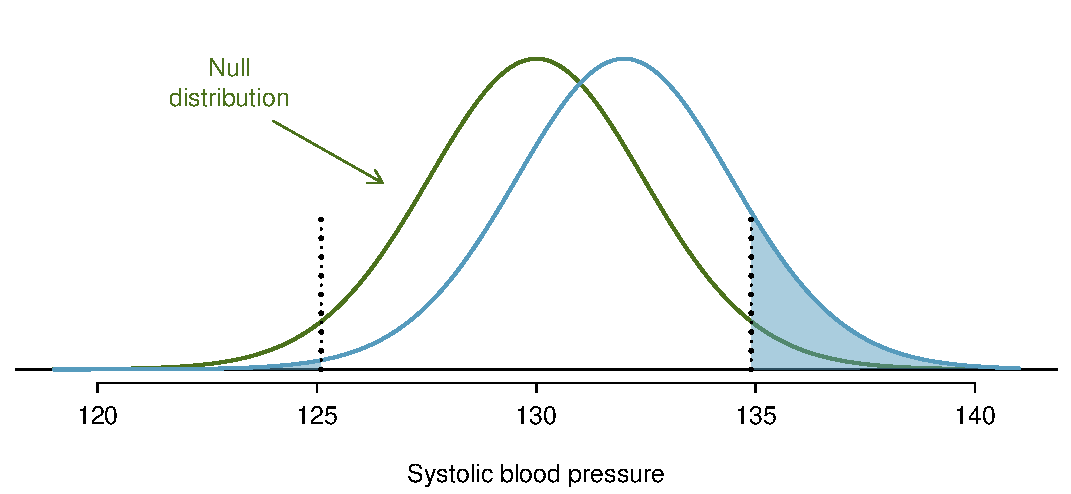
\includegraphics[width=\textwidth]{ch_inference_foundations_oi_biostat/figures/power132And141/power132And141}
\caption{The sampling distribution of $\overline{x}$ under two scenarios. Left: $N(130, 2.5)$. Right: $N(132, 2.5)$, and the shaded areas in this distribution represent the power of the test.}
\label{power132And141}
\end{figure}

The probability of rejecting the null hypothesis is called the \term{power}. The power varies depending on what the supposed the truth might be. In Example~\ref{computePowerIfMuIs132AndMu0Is130}, the difference between the null value and the supposed true mean was relatively small, so the power was also small: only 0.126. However, when the truth is far from the null value, where the standard error is used as a measure of what is far, the power tends to increase.

\begin{exercise}
Suppose the true sampling distribution of $\overline{x}$ is centered at 140. That is, $\overline{x}$ comes from $N(140, 2.5)$. What would the power be under this scenario? It may be helpful to draw $N(140, 2.5)$ and shade the area representing power on Figure~\ref{power132And141}; use the same cutoff values identified in Example~\ref{computePowerIfMuIs132AndMu0Is130}.\footnote{Draw the distribution $N(140, 2.5)$, then find the area below 125.1 (about zero area) and above 134.9 (about 0.979). If the true mean is 140, the power is about 0.979.}
\end{exercise}

\begin{exercise}
If the power of a test is 0.979 for a particular mean, what is the Type 2 Error rate for this mean?\footnote{The Type 2 Error rate represents the probability of failing to reject the null hypothesis. Since the power is the probability that the null hypothesis is rejected, the Type 2 Error rate will be $1-0.979 = 0.021$.}
\end{exercise}

\begin{exercise}
Provide an intuitive explanation for why it is more likely to reject $H_0$ when the true mean is further from the null value.\footnote{Answers may vary a little. When the truth is far from the null value, the point estimate also tends to be far from the null value, making it easier to detect the difference and reject $H_0$.}
\end{exercise}

\subsection{Statistical significance versus practical significance}

When the sample size becomes larger, point estimates become more precise and any real differences in the mean and null value become easier to detect and recognize. Even a very small difference would likely be detected with a large enough sample. Sometimes researchers will decide to take such large samples that even the slightest difference is detected. While the difference is \term{statistically significant}, it might not be \term{practically significant}.

Statistically significant differences are sometimes so minor that they are not practically relevant. This is especially important to research: if a study is conducted, the goal of the study is to find a meaningful and useful result. Researchers do not want to spend money and resources finding results that hold no practical and applicable value.

The role of a statistician or a scientist in conducting a study often includes planning the size of the study and determining the value of $\alpha$. They might first consult experts or scientific literature to learn what would be the smallest meaningful difference from the null value. They also would obtain some reasonable estimate for the standard deviation. With these important pieces of information, a sufficiently large sample size would be chosen so that the power for the meaningful difference is perhaps 80\% or 90\%. While larger sample sizes may still be used, statisticians in practice might advise against it in some cases, especially in sensitive areas of research. Statistical rigor in hypothesis testing is absolutely important, but many of these tests must also stand up to practical significance in the real world within application and relevance. 









%%%%%%%%%%%%%%HERE IS THE COMMENT%%%%%%%%%%%%%%%%%%%%%%%%%%%%
%%%%%%%%%%%%%%HERE IS THE COMMENT%%%%%%%%%%%%%%%%%%%%%%%%%%%%
%%%%%%%%%%%%%%HERE IS THE COMMENT%%%%%%%%%%%%%%%%%%%%
%%%%%%%%%%%%%%HERE IS THE COMMENT%%%%%%%%%%%%%%%%%%%%%%%%%%%%
-----------------------------------------------------------------------------------------------------------------------------------------------------

%%% Use for an example/exercise
\begin{comment}

\subsection{One sample $t$-confidence intervals}
\label{oneSampleTConfidenceIntervals}

\index{data!dolphins and mercury|(}

Dolphins are at the top of the oceanic food chain, which causes dangerous substances such as mercury to concentrate in their organs and muscles. This is an important problem for both dolphins and other animals, like humans, who occasionally eat them. For instance, this is particularly relevant in Japan where school meals have included dolphin at times.
\setlength{\captionwidth}{86mm}

\begin{figure}[h]
\centering
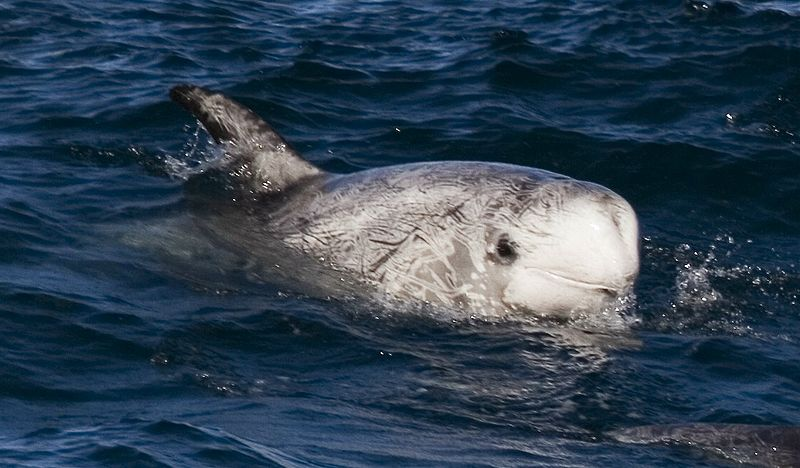
\includegraphics[width=0.8\textwidth]{ch_inference_foundations_oi_biostat/figures/rissosDolphin/rissosDolphin.jpg}  \\
\addvspace{2mm}
\begin{minipage}{\textwidth}
   \caption[rissosDolphinPic]{A Risso's dolphin.\vspace{-1mm} \\
   -----------------------------\vspace{-2mm}\\
   {\footnotesize Photo by Mike Baird (\oiRedirect{textbook-bairdphotos_com}{www.bairdphotos.com}). \oiRedirect{textbook-CC_BY_2}{CC~BY~2.0~license}.}\vspace{-8mm}}
   \label{rissosDolphin}
\end{minipage}
\vspace{3mm}
\end{figure}
\setlength{\captionwidth}{\mycaptionwidth}

Here we identify a confidence interval for the average mercury content in dolphin muscle using a sample of 19 Risso's dolphins from the Taiji area in Japan.\footnote{Taiji was featured in the movie \emph{The Cove}, and it is a significant source of dolphin and whale meat in Japan. Thousands of dolphins pass through the Taiji area annually, and we will assume these 19 dolphins represent a simple random sample from those dolphins. Data reference: Endo T and Haraguchi K. 2009. High mercury levels in hair samples from residents of Taiji, a Japanese whaling town. Marine Pollution Bulletin 60(5):743-747.} The data are summarized in Table~\ref{summaryStatsOfHgInMuscleOfRissosDolphins}. The minimum and maximum observed values can be used to evaluate whether or not there are obvious outliers or skew.

\begin{table}[h]
\centering
\begin{tabular}{ccc cc}
\hline
$n$ & $\overline{x}$ & $s$ & minimum & maximum \\
19   & 4.4	  & 2.3  & 1.7	       & 9.2 \\
\hline
\end{tabular}
\caption{Summary of mercury content in the muscle of 19 Risso's dolphins from the Taiji area. Measurements are in $\mu$g/wet g (micrograms of mercury per wet gram of muscle).}
\label{summaryStatsOfHgInMuscleOfRissosDolphins}
\end{table}

\begin{example}{Are the independence and normality conditions satisfied for this data~set?}
The observations are a simple random sample and consist of less than 10\% of the population, therefore independence is reasonable. The summary statistics in Table~\ref{summaryStatsOfHgInMuscleOfRissosDolphins} do not suggest any skew or outliers; all observations are within 2.5 standard deviations of the mean. Based on this evidence, the normality assumption seems reasonable.
\end{example}

In the normal model, we used $z^{\star}$ and the standard error to determine the width of a confidence interval. We revise the confidence interval formula slightly when using the $t$-distribution:
\begin{eqnarray*}
\overline{x} \ \pm\  t^{\star}_{df}SE
\end{eqnarray*}
\marginpar[\raggedright\vspace{-9mm}

$t^{\star}_{df}$\vspace{1mm}\\\footnotesize Multiplication\\factor for\\$t$ conf. interval]{\raggedright\vspace{-9mm}

$t^{\star}_{df}$\vspace{1mm}\\\footnotesize Multiplication\\factor for\\$t$ conf. interval}The sample mean and estimated standard error are computed just as before ($\overline{x} = 4.4$ and $SE = s/\sqrt{n} = 0.528$). The value $t^{\star}_{df}$ is a cutoff we obtain based on the confidence level and the $t$-distribution with $df$ degrees of freedom. Before determining this cutoff, we will first need the degrees of freedom.

\begin{termBox}{\tBoxTitle{Degrees of freedom for a single sample}
If the sample has $n$ observations and we are examining a single mean, then we use the $t$-distribution with $df=n-1$ degrees of freedom.}
\end{termBox}

In our current example, we should use the $t$-distribution with $df=19-1=18$ degrees of freedom. Then identifying $t_{18}^{\star}$ is similar to how we found $z^{\star}$. 
\begin{itemize}
\setlength{\itemsep}{0mm}
\item For a 95\% confidence interval, we want to find the cutoff $t^{\star}_{18}$ such that 95\% of the $t$-distribution is between -$t^{\star}_{18}$ and $t^{\star}_{18}$.
\item We look in the $t$-table on page~\pageref{tTableSample}, find the column with area totaling 0.05 in the two tails (third column), and then the row with 18 degrees of freedom: $t^{\star}_{18} = 2.10$.
\end{itemize}
Generally the value of $t^{\star}_{df}$ is slightly larger than what we would get under the normal model with~$z^{\star}$.

Finally, we can substitute all our values into the confidence interval equation to create the 95\% confidence interval for the average mercury content in muscles from Risso's dolphins that pass through the Taiji area:
\begin{eqnarray*}
\overline{x} \ \pm\  t^{\star}_{18}SE
	\quad \to \quad
4.4 \ \pm\  2.10 \times 0.528
	\quad \to \quad
(3.29, 5.51)
\end{eqnarray*}
We are 95\% confident the average mercury content of muscles in Risso's dolphins is between 3.29 and 5.51 $\mu$g/wet gram, which is considered extremely high.

\index{data!dolphins and mercury|)}

\begin{termBox}{\tBoxTitle{Finding a $t$-confidence interval for the mean}
Based on a sample of $n$ independent and nearly normal observations, a confidence interval for the population mean is
\begin{eqnarray*}
\overline{x} \ \pm\  t^{\star}_{df}SE
\end{eqnarray*}
where $\overline{x}$ is the sample mean, $t^{\star}_{df}$ corresponds to the confidence level and degrees of freedom, and $SE$ is the standard error as estimated by the sample.}
\end{termBox}

\textC{\pagebreak}

\begin{exercise} \label{croakerWhiteFishPacificExerConditions}
\index{data!white fish and mercury|(}
The FDA's webpage provides some data on mercury content of fish.\footnote{\oiRedirect{textbook-fda_mercury_in_fish_2010}{www.fda.gov/food/foodborneillnesscontaminants/metals/ucm115644.htm}} Based on a sample of 15 croaker white fish (Pacific), a sample mean and standard deviation were computed as 0.287 and 0.069 ppm (parts per million), respectively. The 15 observations ranged from 0.18 to 0.41 ppm. We will assume these observations are independent. Based on the summary statistics of the data, do you have any objections to the normality condition of the individual observations?\footnote{There are no obvious outliers; all observations are within 2 standard deviations of the mean. If there is skew, it is not evident. There are no red flags for the normal model based on this (limited) information, and we do not have reason to believe the mercury content is not nearly normal in this type of fish.}
\end{exercise}

\begin{example}{Estimate the standard error of $\overline{x}=0.287$ ppm using the data summaries in Guided Practice~\ref{croakerWhiteFishPacificExerConditions}. If we are to use the $t$-distribution to create a 90\% confidence interval for the actual mean of the mercury content, identify the degrees of freedom we should use and also find $t^{\star}_{df}$.}
\label{croakerWhiteFishPacificExerSEDFTStar}
The standard error: $SE = \frac{0.069}{\sqrt{15}} = 0.0178$. Degrees of freedom: $df = n - 1 = 14$.

Looking in the column where two tails is 0.100 (for a 90\% confidence interval) and row $df=14$, we identify $t^{\star}_{14} = 1.76$.
\end{example}

\begin{exercise}
Using the results of Guided Practice~\ref{croakerWhiteFishPacificExerConditions} and Example~\ref{croakerWhiteFishPacificExerSEDFTStar}, compute a 90\% confidence interval for the average mercury content of croaker white fish (Pacific).\footnote{$\overline{x} \ \pm\ t^{\star}_{14} SE \ \to\  0.287 \ \pm\  1.76\times 0.0178\ \to\ (0.256, 0.318)$. We are 90\% confident that the average mercury content of croaker white fish (Pacific) is between 0.256 and 0.318 ppm.}

\index{data!white fish and mercury|)}

\end{exercise}

\end{comment} 
%%%